%----------------------------------------------------------------------------------------
%	PACKAGES AND THEMES
%----------------------------------------------------------------------------------------
\PassOptionsToPackage{table}{xcolor}
\documentclass[aspectratio=169,xcolor=dvipsnames,11pt]{beamer}
\usetheme{SimplePlusAIC}
\usepackage{amsmath}
\usepackage{animate}
\usepackage{hyperref}
\usepackage{cleveref}
\usepackage{caption}
\usepackage{graphicx} % Allows including images
%\usepackage{subfig}
\usepackage{subcaption}
\usepackage{booktabs} % Allows the use of \toprule, \midrule and  \bottomrule in tables
\usepackage{svg} %allows using svg figures
\usepackage{tikz}
\usepackage{makecell}
\usepackage{multirow}
\usepackage{appendixnumberbeamer}
\usepackage{wrapfig}
\usepackage{verbatim}
\usepackage{tcolorbox}
%\usepackage[dvipsnames]{xcolor}

\usepackage{hhline}
\usepackage{relsize}
\usepackage{bm}
%Select the Epilogue font (requires luaLatex or XeLaTex compilers)
%\setsansfont{Epilogue}[
  %  Path=./epilogueFont/,
  %  Scale=0.9,
  %  Extension = .ttf,
   % UprightFont=*-Regular,
   % BoldFont=*-Bold,
   % ItalicFont=*-Italic,
    %BoldItalicFont=*-BoldItalic
    %]
    \usefonttheme[onlymath]{serif}
% \usepackage{ eulervm } % Euler VM as math serif font

\newcommand*{\defeq}{\stackrel{\text{def}}{=}}
\newcommand{\grad}{\nabla}
\newcommand{\lap}{\Delta}
\newcommand{\weaklyto}{\rightharpoonup}
\newcommand{\weakstar}{\stackrel{*}\rightharpoonup}
\newcommand{\cts}{\hookrightarrow}
\newcommand{\ctsDense}{\xhookrightarrow{d}}
\newcommand{\ctsCompact}{\xhookrightarrow{c}}
\newcommand{\E}{\mathbb{E}}
\newcommand{\pP}{\mathbb{P}}
\newcommand{\R}{\mathbb{R}}
\newcommand{\ER}{\overline{\mathbb{R}}}
\newcommand{\cR}{\mathcal{R}}
\newcommand{\cJ}{\mathcal{J}}
\newcommand{\cG}{\mathcal{G}}
\newcommand{\CVaR}{\textup{CVaR}}
\newcommand{\D}{\textup{ d}}
\newcommand{\dd}{\mathrm{d}}
\newcommand{\fa}{\text{for all }}
\DeclareMathOperator*{\essinf}{\vphantom{p}ess\,inf}
\DeclareMathOperator{\sigmoid}{expit} % a.k.a. logistic sigmoid

\usepackage[ruled,vlined,algo2e]{algorithm2e}
\crefname{algocf}{algorithm}{algorithms}
 \usepackage{caption}

\usepackage{tcolorbox}  % For fancy boxes
\usepackage{lipsum}     % For dummy text

% Define a custom style for the box
\tcbuselibrary{skins, breakable}
\newtcolorbox[auto counter, number within=section]{roundedshadowbox}[2][]{
    colback=white, % Background color (kept white)
    colframe=black, % Border color
    boxrule=0.5pt, % Border thickness
    arc=5mm, % Rounded corners
    shadow=true, % Drop shadow effect
    width=\linewidth, % Full width box
    title=#2, % Title text
    #1 % Additional options (e.g., width override)
}

\usepackage{pgfplots}
\pgfplotsset{compat=1.18}

%\PassOptionsToPackage{table}{xcolor}
%\documentclass[aspectratio=169,xcolor=dvipsnames,11pt]{beamer}
%\usetheme{SimplePlusAIC}
%\usepackage{amsmath}
%\usepackage{hyperref}
%\usepackage{cleveref}
%\usepackage{caption}
%\usepackage{graphicx} % Allows including images
%\usepackage{subcaption}
%\usepackage{booktabs} % Allows the use of \toprule, \midrule and  \bottomrule in tables
%\usepackage{svg} %allows using svg figures
%\usepackage{tikz}
%
%\usepackage{pgfplots}
%\pgfplotsset{compat=1.18}
%
%\usepackage{makecell}
%\usepackage{multirow}
%\usepackage{appendixnumberbeamer}
%\usepackage{wrapfig}
%\usepackage{verbatim}
%\usepackage{tcolorbox}
%\usepackage{hhline}
%\usepackage{relsize}
%\usepackage{bm}
%
%\usefonttheme[onlymath]{serif}
%    
\newcommand{\C}{\mathbb C}

%
%%\font\nullfont=cmr10
%
%\usepackage{tcolorbox}  % For fancy boxes
%\usepackage{lipsum}     % For dummy text
%
%% Define a custom style for the box
%\tcbuselibrary{skins, breakable}
%\newtcolorbox[auto counter, number within=section]{roundedshadowbox}[2][]{
%    colback=white, % Background color (kept white)
%    colframe=black, % Border color
%    boxrule=0.5pt, % Border thickness
%    arc=5mm, % Rounded corners
%    shadow=true, % Drop shadow effect
%    width=\linewidth, % Full width box
%    title=#2, % Title text
%    #1 % Additional options (e.g., width override)
%}


%----------------------------------------------------------------------------------------
%	TITLE PAGE
%----------------------------------------------------------------------------------------

\title[LVPP Course I]{The Latent Variable Proximal Point Method I: Introduction and Preliminary Results
 }
% \title[\quad\quad\quad LVPP Course I]{The Latent Variable Proximal Point Method I: Introduction and Preliminary Results
% } 
  % The short title appears at the bottom of every slide, the full title is only on the title page
%\subtitle{Subtitle}

\author{\small{\bf Thomas M. Surowiec}}

\institute[T.M. Surowiec]{Department of Numerical Analysis and Scientific Computing \newline Simula Research Laboratory \newline Oslo, Norway}
% Your institution as it will appear on the bottom of every slide, maybe shorthand to save space


\date{{\footnotesize 
K\'acov, Czechia, 15-20 June 2025}}
%----------------------------------------------------------------------------------------
%	PRESENTATION SLIDES
%----------------------------------------------------------------------------------------

\begin{document}
%
%{
%\setbeamertemplate{background canvas}{}
%\frame{\titlepage}
%}

\begin{frame}[plain]
%\setbeamertemplate{footline}{}
\titlepage
\end{frame}

\begin{frame}{Overview}
\tableofcontents
\end{frame}

\section{Motivation and context}\label{sec:motivation}
%\begin{frame}{Dirichlet's Principle}
%    \begin{enumerate}
%        \item History
%            \begin{enumerate}
%                \item Who invented it, when did it get its name, etc.
%            \end{enumerate}
%        \item Modern interpretation and a first variational inequality
%            \begin{enumerate}
%                \item Derivation of a variational inequality
%                    \begin{enumerate}
%                        \item The feasible set is nonempty, closed, and convex
%                        \item Existence via direct method
%                        \item The objective function is G\^{a}teaux differentiable
%                        \item Derivation of the VI
%                    \end{enumerate}
%            \end{enumerate}
%        \item Reformulation as a variational equation
%            \begin{enumerate}
%                \item Using a clever test function
%                \item Use lifting discussion see Chouly 2023, Poisson.
%            \end{enumerate}
%    \end{enumerate}
%\end{frame}


\begin{frame}{Dirichlet's Principle}

  \begin{minipage}{0.48\textwidth}
  \begin{beamercolorbox}[rounded=true, shadow=true, wd=\textwidth]{block body}
 \textit{The solution to Poisson's equation is the minimizer of a certain energy functional.}\\
  
  \visible<2->{Early observations due to Thomson and Gau\ss.}\\
  
  \visible<3->{Riemann named it after his teacher Dirichlet.}\\
  
  \visible<4->{Hilbert justified Riemann's use of Dirichlet's principle,\\ invents the Direct Method (1900-1905).}
     \end{beamercolorbox}
    \end{minipage}\hspace*{1.75cm}
    \begin{minipage}{0.3\textwidth}
  \centering
 \begin{figure}
  \centering\vspace{1ex}
  \only<1-3>{\begin{minipage}[b]{0.45\textwidth}
    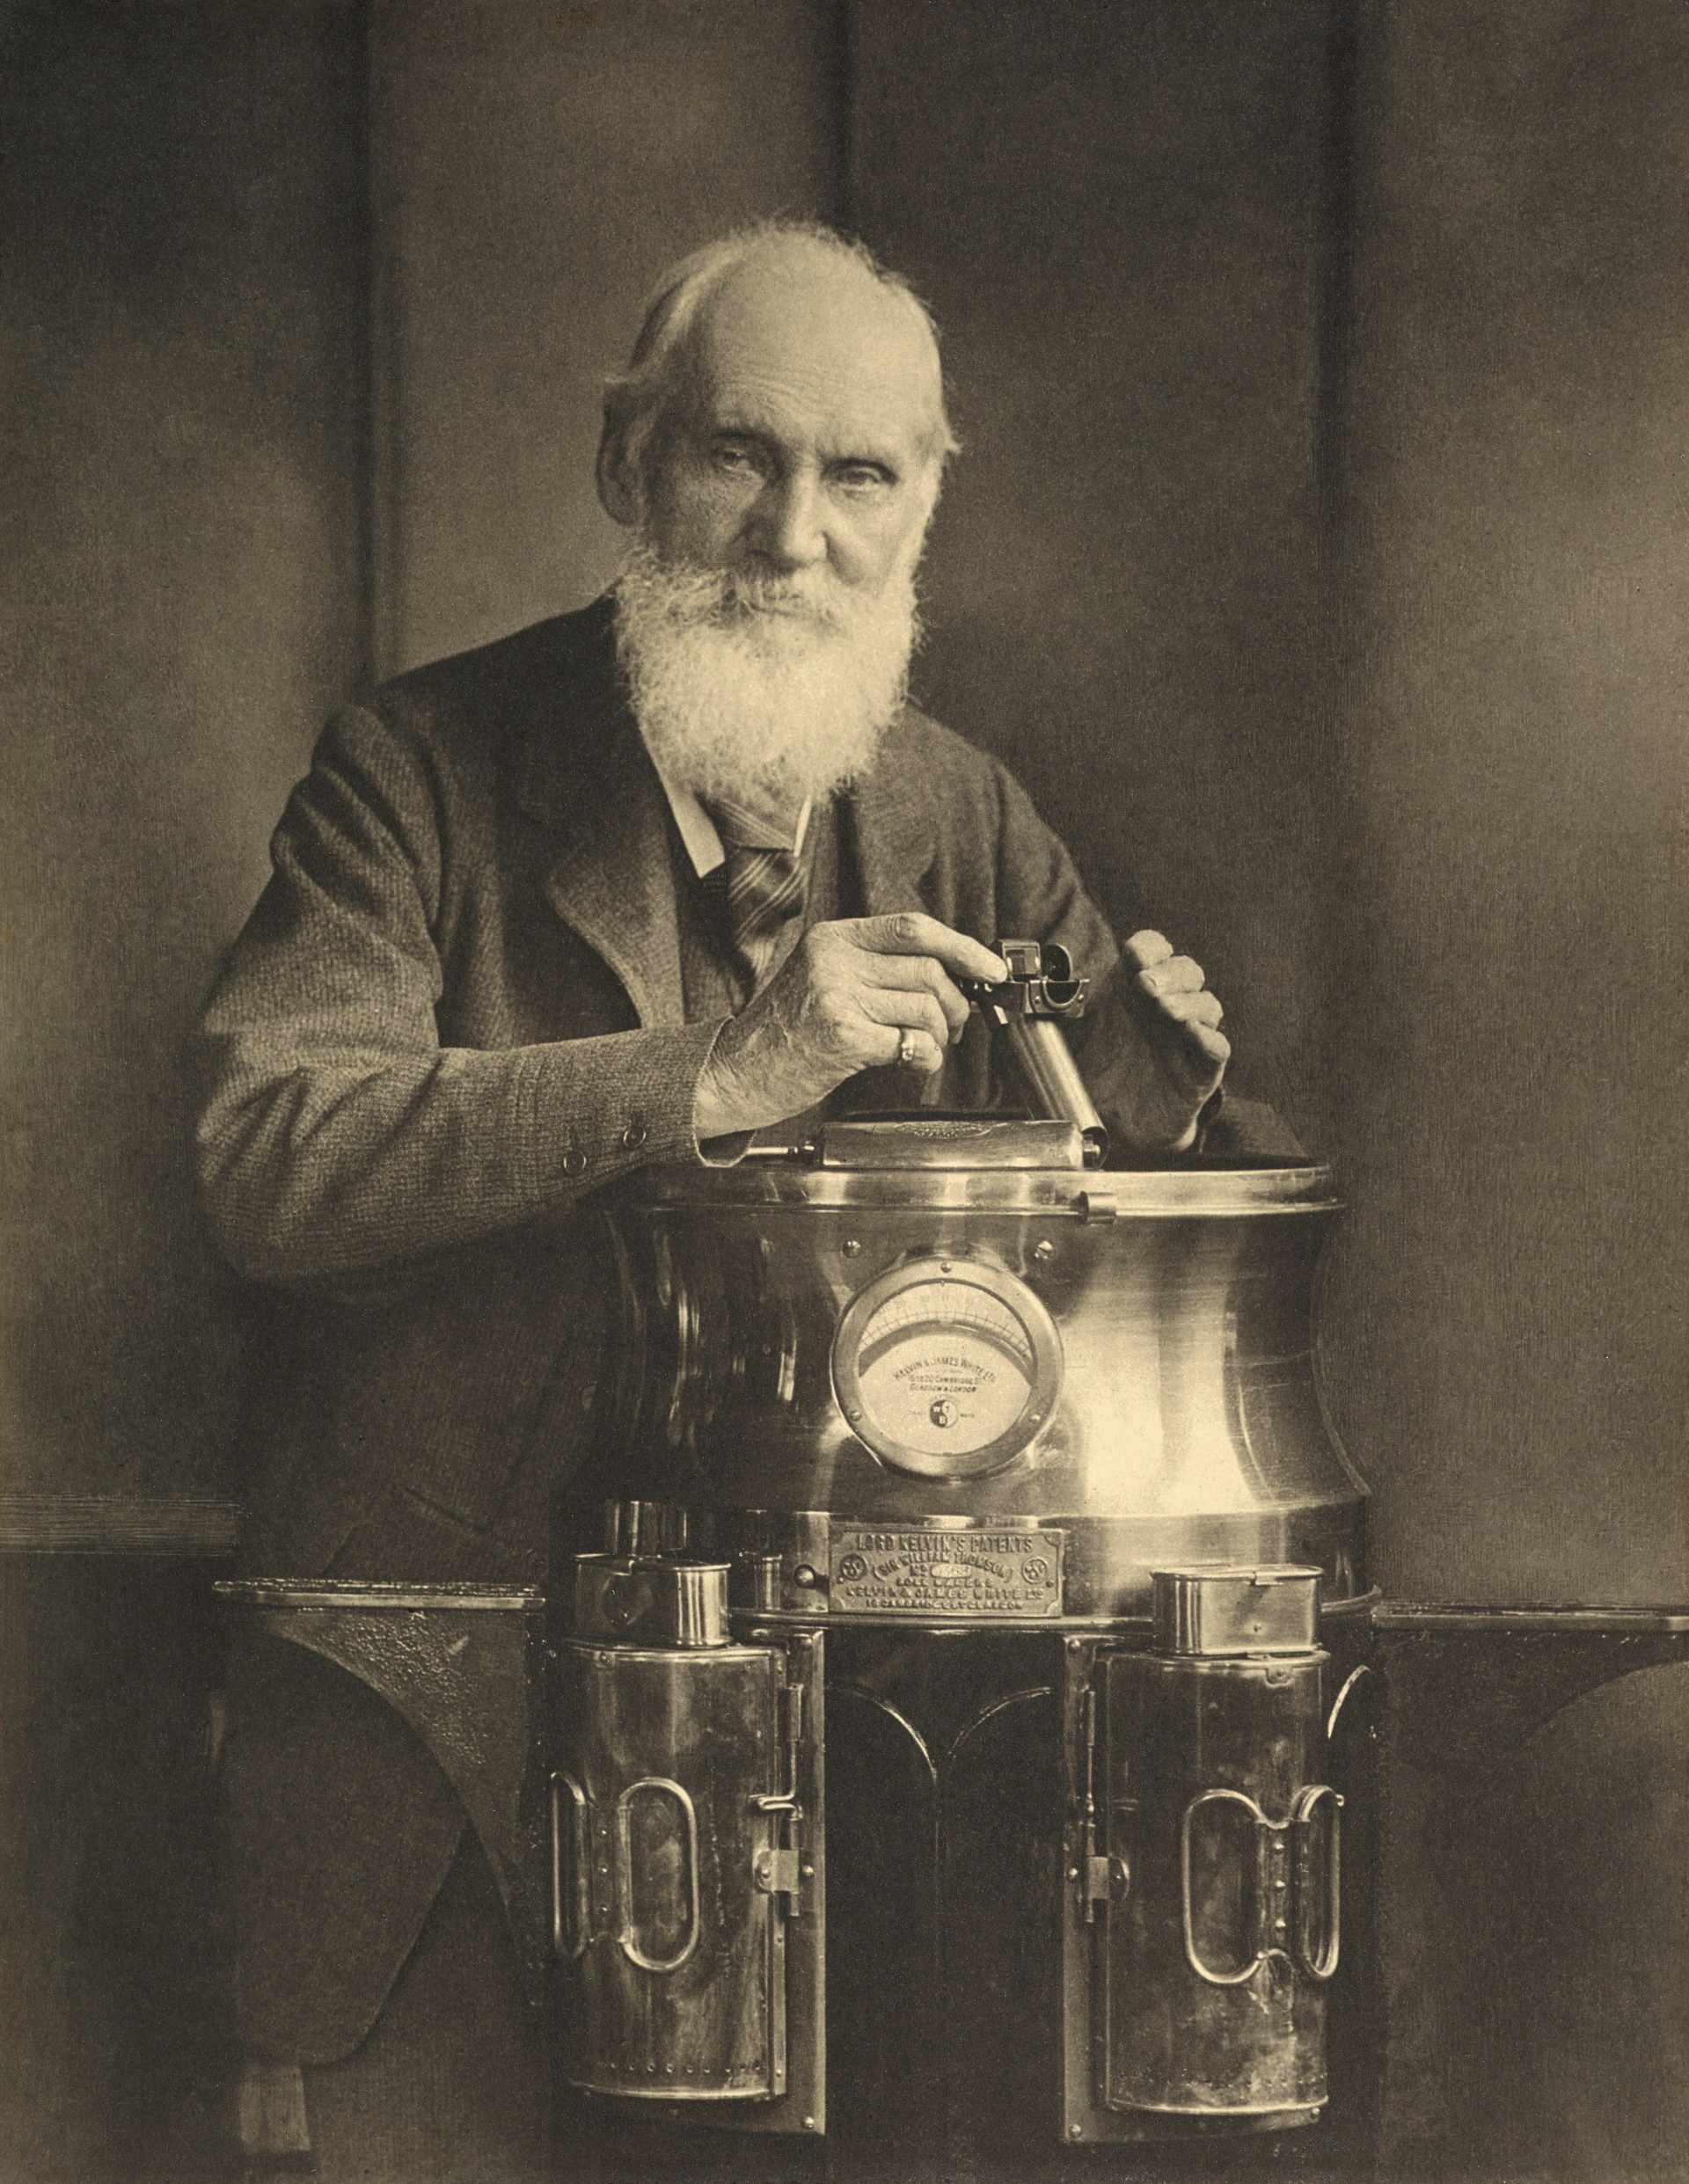
\includegraphics[width=\linewidth]{figures/kelvin.jpg}
    \captionof*{figure}{\tiny W. Thomson}
  \end{minipage}}%
   \only<4->{\begin{minipage}[b]{0.43\textwidth}
    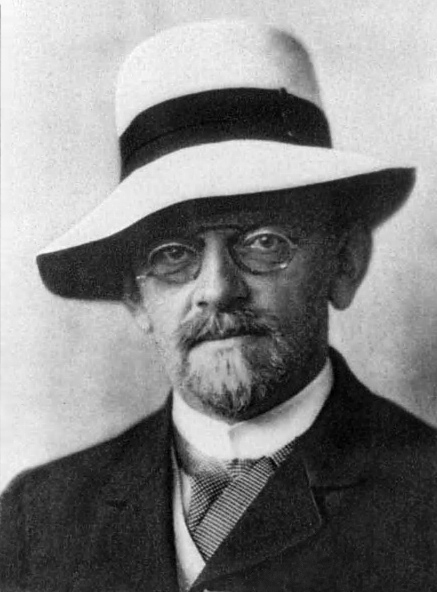
\includegraphics[width=\linewidth]{figures/Hilbert.jpg}
    \captionof*{figure}{\tiny \alert{D. Hilbert}}
  \end{minipage}}
  \hfill
  \begin{minipage}[b]{0.455\textwidth}
    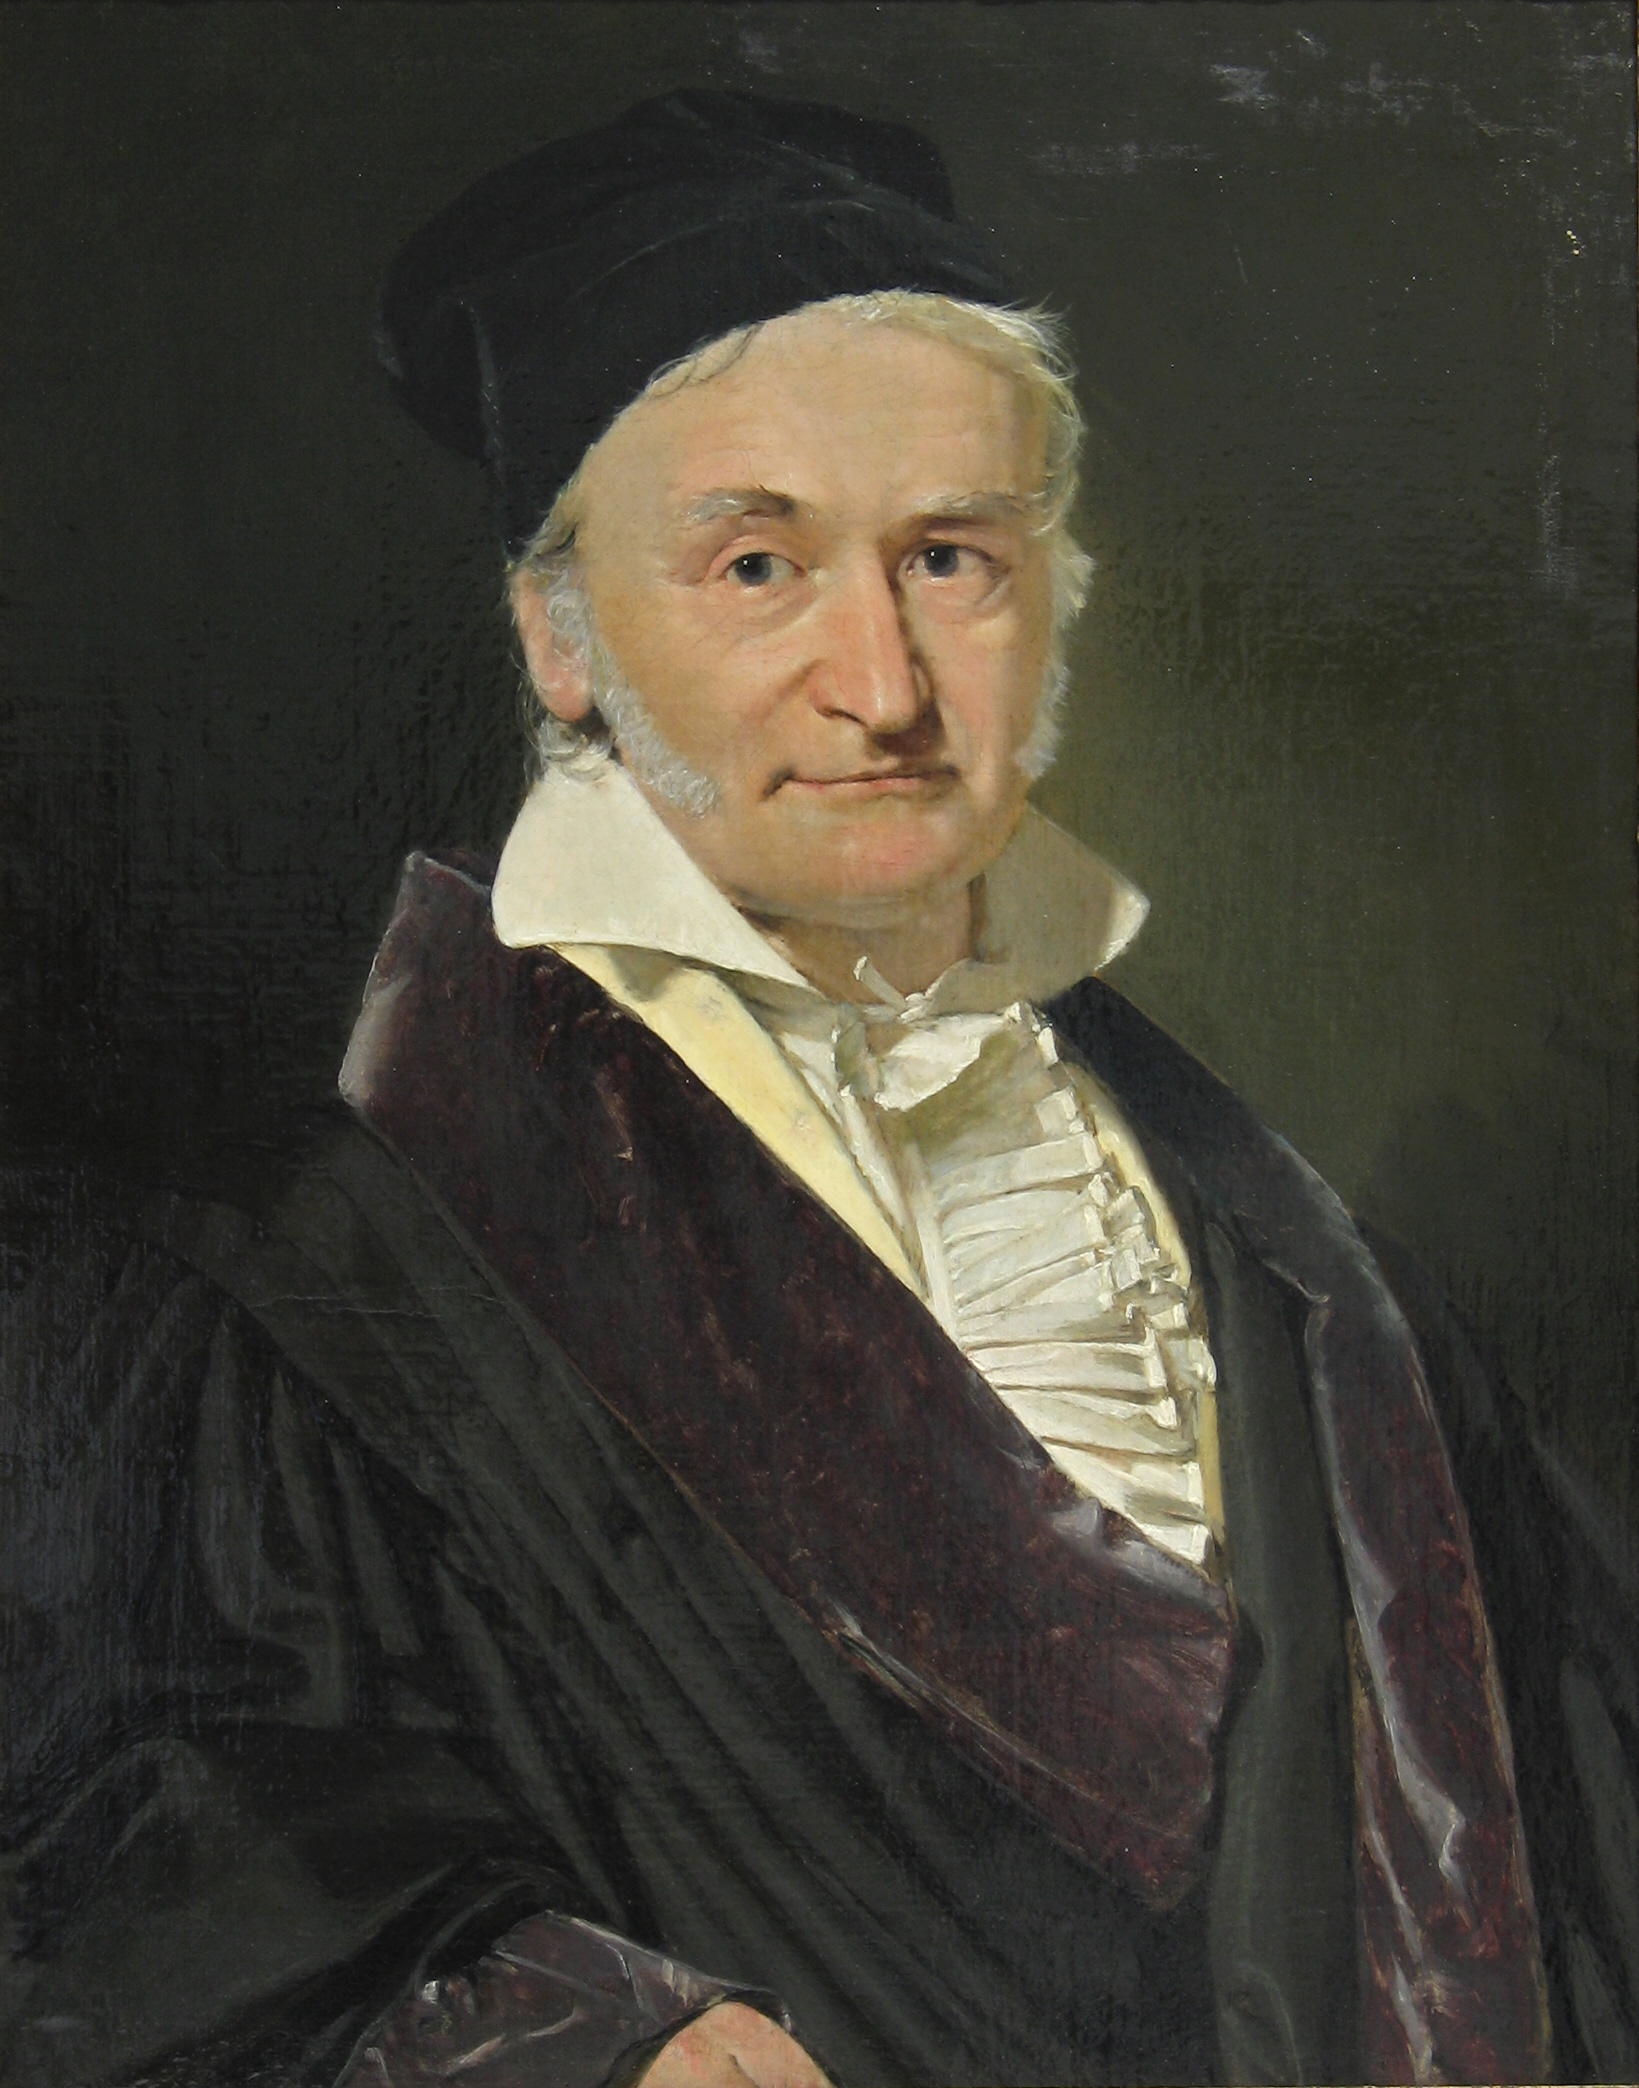
\includegraphics[width=\linewidth]{figures/gauss.jpg}
    \captionof*{figure}{\tiny C.F. Gau\ss }
  \end{minipage}
  \vspace{1em}
  \begin{minipage}[b]{0.45\textwidth}
    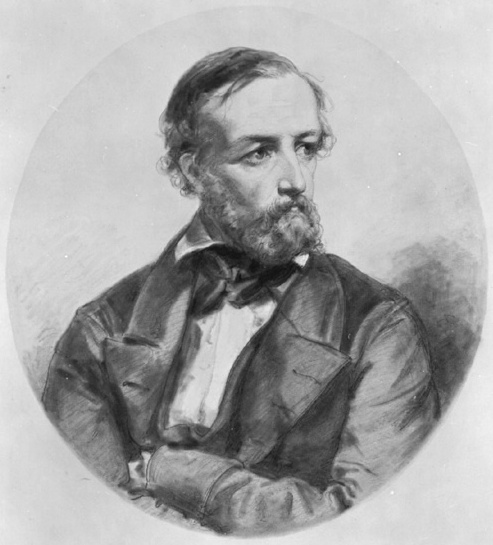
\includegraphics[width=\linewidth]{figures/dirichlet.jpg}
    \captionof*{figure}{\tiny P.G.L. Dirichlet}
  \end{minipage}
  \hfill
  \begin{minipage}[b]{0.45\textwidth}
    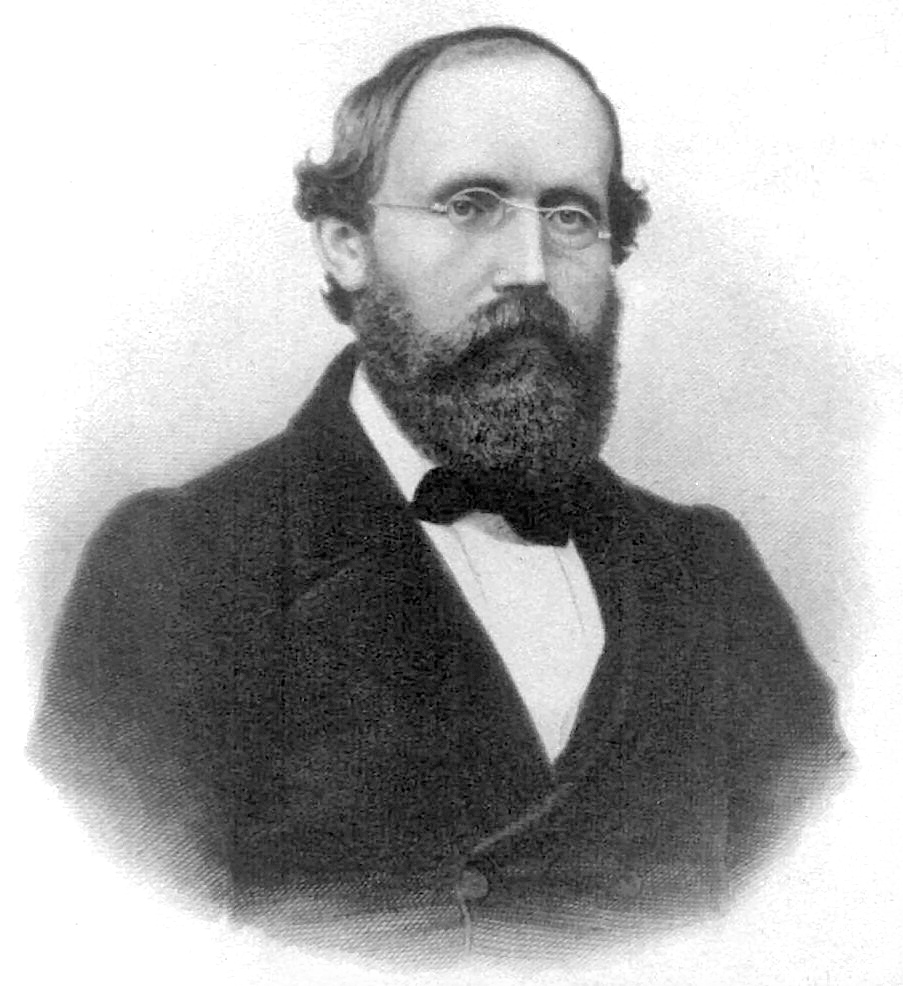
\includegraphics[width=\linewidth]{figures/riemann.jpg}
    \captionof*{figure}{\tiny B. Riemann}
  \end{minipage}
\end{figure}
    \end{minipage}
\end{frame}

\begin{frame}\frametitle{Dirichlet's Principle: Modern Form}
% We seek a minimizer $u$ of the energy functional:
% \begin{equation*}
% 	E(v)
% 	=
% 	\frac{1}{2}
% 	\int_\Omega |\nabla v|^2 \dd x
% 	-
% 	\int_\Omega v f \dd x
% 	\,,
% \end{equation*}
% over the \textbf{closed convex cone} defined by  
% \[
% K = \{ v \in H^1_0(\Omega) \mid v \geq 0 \text{~a.e.}\}.
% \] 
% (Displacements $v \ge 0$, the obstacle)

 \begin{beamercolorbox}[rounded=true, shadow=true, wd=\textwidth]{block body}
\visible<1->{For any $f\in L^2(\Omega)$ and $g\in H^{1/2}(\Gamma)$, the (weak) solution of Poisson's equation over an open bounded Lipschitz domain $\Omega \subset \mathbb{R}^n$ with boundary $\Gamma$
 \begin{equation}
 \label{eq:PoissonEquation}\tag{Poisson Problem}
 	-\Delta u = f
 	\quad \text{in~} \Omega,
 	\qquad
 	u = g \quad \text{on~} \Gamma,
 \end{equation}}\visible<2->{
 is the \textbf{$H^1(\Omega)$-minimizer} of the total energy functional,
 \begin{equation}
 \label{eq:DirichletEnergy}\tag{Dirichlet Energy}
 	E(v)
 	=
 	\frac{1}{2}
 	\int_\Omega |\nabla v|^2 \dd x
 	-
 	\int_\Omega f v \dd x
 	\,,
 \end{equation}}\visible<3->{
 when confined to the \textbf{constraint set} $H^1_g(\Omega) = g + H^1_0(\Omega) = \{ v \in H^1(\Omega) \mid v = g \text{~on~} \partial \Omega\}$.}
\end{beamercolorbox}

\visible<4->{
 \begin{beamercolorbox}[rounded=true, shadow=true, wd=\textwidth]{block title}\centering
 We sketch the proof. The arguments extend to much more complicated examples!
 \end{beamercolorbox}
}
\end{frame}

\begin{frame}\frametitle{The Direct Method}

 \begin{beamercolorbox}[rounded=true, shadow=true, wd=\textwidth]{block body}
 There are a few basic steps
 \begin{enumerate}
 \item Start with a minimizing sequence $\left\{v_k\right\}$ meaning  \[\inf_{v \in H^1_g(\Omega)} E(v) = \liminf_{k \to +\infty} E(v_k).\] 
 \item For some topology $\tau$, show $\left\{v_k\right\}$ admits a $\tau$-convergent subsequence $\left\{v_{k_l}\right\}$ to some $\bar{v}$.
 \item Argue that $\bar{v}$ is a feasible point, i.e. $\bar{v} \in H^1_g(\Omega)$.
 \item Show that $E$ is $\tau$-lower semicontinuous. 
 \end{enumerate}
 \end{beamercolorbox}

\visible<2->{
 \begin{beamercolorbox}[rounded=true, shadow=true, wd=\textwidth]{block title}
% This works because
  \[
 \inf_{v \in H^1_g(\Omega)} E(v) = \liminf_{k \to +\infty} E(v_k) =  \liminf_{l \to +\infty} E(v_{k_l}) \ge E(\bar{v}) \ge  \inf_{v \in H^1_g(\Omega)} E(v).
 \]
  \end{beamercolorbox}}
 
\end{frame}

\begin{frame}\frametitle{The Direct Method}
 \begin{beamercolorbox}[rounded=true, shadow=true, wd=\textwidth]{block body}
 \visible<1->{We would like to \alert{prove} the existence of a solution to the optimization problem:
 \[
 \inf_{u \in H^1_g(\Omega)} E(u).
 \]
We use the \alert{Direct Method of the Calculus of Variations}. For simplicity $g \equiv 0$, $f \ne 0$.}
 \end{beamercolorbox}
 
 \visible<2->{
  \begin{beamercolorbox}[rounded=true, shadow=true, wd=\textwidth]{block body}
% \begin{enumerate}
% \item 
\visible<2->{$E$ is not bound from below here. However,}
\visible<3->{for any $v \in H^1_0(\Omega)$, $E(v)$ is finite and 
 \[
 E(v) \ge \frac{1}{2} \| \nabla v \|^2_{L^2} - \| v \|_{L^2} \|f\|_{L^2} \ge \frac{1}{2} \| \nabla v \|^2_{L^2} - C \|\nabla v \|_{L^2} \| f \|_{L^2}
 \]}\vspace*{-1ex}
% \item 

 \visible<4->{This means, if $\|v\|_{H^1_0} \to +\infty$, then $E(v) \to +\infty$, i.e., $E$ is \alert{$H^1_0(\Omega)$-coercive}.\medskip
% \item 
 }
 
 \visible<5->{
 Thus, $N_0 := \left\{ v \in H^1_0(\Omega) \left| E(v) \le E(v_0) \right.\right\}$ for any $v_0 \in H^1_0(\Omega)$ is \alert{bounded in $H^1_0(\Omega)$}.}
% \end{enumerate}
 \end{beamercolorbox}
 }
\end{frame}

\begin{frame}\frametitle{The Direct Method}
 \visible<1->{\begin{beamercolorbox}[rounded=true, shadow=true, wd=\textwidth]{block body}
\visible<1->{If  $\{v_k\} \subset H^1_0(\Omega)$ is a minimizing sequence, then $v_k \in N_0$ for large $k$.\medskip

Thus, $\{v_k\}$ is a \alert{bounded sequence}.\medskip
}

\visible<2->{$H^1_0(\Omega)$ is Hilbert $\Rightarrow$ bounded sequences admit \alert{weakly convergent subsequences}.\medskip

\visible<3->{Hence, there exists $\{v_{k_l}\} \subset \{v_k\}$ and $\bar{v} \in H^1_0(\Omega)$ such that $v_{k_l} \rightharpoonup \bar{v}$ (weakly in $H^1_0(\Omega))$.

\rule{\linewidth}{0.4pt}\medskip

}


\visible<4->{
$E$ is the sum of a convex continuous function and a continuous linear functional.\medskip
}

\visible<5->{
 We can thus easily show that $E$ is \alert{weakly lower-semicontinuous}, meaning
 \[
 \forall v \in H^1_0(\Omega), \forall \{v_k\} \subset H^1_0(\Omega) : v_k \rightharpoonup v \quad\text{ we have }\quad \liminf_{k \to +\infty} E(v_k) \ge E(v).
 \]
}\vspace{-2ex}

\visible<6->{
This completes the proof, i.e., $u = \bar{v}$ is a minimizer of $E$ over $H^1_0(\Omega)$.
}
}
 \end{beamercolorbox}
 }
\end{frame}

\begin{frame}\frametitle{Optimality Conditions}
 \visible<1->{\begin{beamercolorbox}[rounded=true, shadow=true, wd=\textwidth]{block body}
  \visible<1->{The objective $E$ is \alert{strongly convex}: There is a $c > 0$ for all $u,v \in H^1_0(\Omega)$ and $\lambda \in [0,1]$
  \[
  E(\lambda u + (1-\lambda) v) \le \lambda E(u) + (1-\lambda) E(v) - c \lambda (1 - \lambda) \| u - v \|^2_{H^1_0}.
  \]
  }\vspace{-2ex}
  
  \visible<2->{
  This makes it easy to show that the minimzer of $E$ is unique. But where's the PDE?
  }\medskip
  
 \visible<3->{
 Observe: 
 \begin{enumerate}
 \item \visible<3->{
  For $v, w \in H^1_g(\Omega)$, $\lambda \in (0,1)$, we have $( \lambda v + (1-\lambda) w)|_{\Gamma} = \lambda g + (1-\lambda) g = g$.
  \item This means the feasible set $H^1_g(\Omega)$ is convex. (Easy to show $\ne\emptyset$ and closed).
 }
\item \visible<4->{
 For any $v \in H^1_g(\Omega)$ and $\tau > 0$ we have 
 \[
 E( u + \tau v) = E(u) + \tau [(\nabla u, \nabla v)_{L^2} - (f,v)_{L^2}] + \frac{\tau^2}{2} \| \nabla v \|^2_{L^2}
 \]
 }\vspace{-3ex}
 \end{enumerate}
 }
 \end{beamercolorbox}}
\end{frame}

\begin{frame}\frametitle{Optimality Conditions}
 \visible<1->{\begin{beamercolorbox}[rounded=true, shadow=true, wd=\textwidth]{block body}
 Consider the definition of our unique minimizer $u$: 
 \[
 E(u) \le E(v) \quad \forall v \in H^1_g(\Omega).
 \]
 
 \visible<2->{
 Since $H^1_g(\Omega)$ is a convex set, $\lambda v + (1-\lambda) u = u + \lambda (v - u) \in H^1_g(\Omega)$ for all $v \in H^1_g(\Omega)$.
 }\medskip
 
  \visible<3->{
  Then for fixed arbitrary $v \in H^1_g(\Omega)$, we have:
  \[
  E(u) \le E(u + \lambda (v - u) ) = E(u) + \lambda [(\nabla u, \nabla [v-u])_{L^2} - (f,v-u)_{L^2}] + \frac{\lambda^2}{2} \| \nabla [v-u] \|^2_{L^2}
  \] }\visible<4->{and hence,
  \[
 \lambda [(\nabla u, \nabla [v-u])_{L^2} - (f,v-u)_{L^2}] \ge o(\lambda) 
  \]}\visible<5->{Divide by $\lambda > 0$ and let $\lambda \to 0$.
  }
 
 \end{beamercolorbox}}
\end{frame}

\begin{frame}\frametitle{A First Variational Inequality}
 \visible<1->{\begin{beamercolorbox}[rounded=true, shadow=true, wd=\textwidth]{block body}
 \visible<1->{The following \alert{variational inequality} characterizes our solution $u$:
 \[
 (\nabla u, \nabla [v-u])_{L^2} \ge  (f,v-u)_{L^2} \quad \forall v \in H^1_g(\Omega)
 \]
 It states: \textit{The direction derivative of $E$ at $u$ in any feasible direction $v - u$ is non-negative.}
 }\medskip
 
\visible<2->{
In this simple example, we have, for any $v \in H^1_g(\Omega)$ and $w \in H^1_0(\Omega)$, $v + w \in H^1_g(\Omega)$.
}\medskip
 
\visible<3->{
This means $u \in H^1_g(\Omega)$ solves
 \[
 (\nabla u, \nabla w)_{L^2} =  (f,w)_{L^2} \quad \forall v \in H^1_0(\Omega),
 \]
 which brings us back to Poisson. (use $u + w$ and $u-w$ in the VI)
 }
  \end{beamercolorbox}}
  
\visible<4->{\begin{beamercolorbox}[rounded=true, shadow=true, wd=\textwidth]{block title}
\centering  But what about more complicated feasible sets?
\end{beamercolorbox}}
\end{frame}

\section{Variational Inequalities}



\begin{frame}{Pointwise Inequality Constraints}
 \visible<1->{\begin{beamercolorbox}[rounded=true, shadow=true, wd=\textwidth]{block body}
Given $u \in H^1(\Omega)$ with $u|_{\Gamma} = g$ we look for solutions satisfying a \alert{pointwise inequality}:
 \[
  u \ge \varphi \quad \text{almost everywhere (a.e.) on } \Omega.
 \]
 Denote this \alert{feasible set} by $K$.
 \end{beamercolorbox}}
 
 \visible<2->{\begin{beamercolorbox}[rounded=true, shadow=true, wd=\textwidth]{block title}
 \centering Are constraints like this even relevant?
 \end{beamercolorbox}
 }
\end{frame}

\begin{frame}\frametitle{The Signorini Problem}
\begin{minipage}{0.55\linewidth}
\visible<1->{
\begin{beamercolorbox}[rounded=true, shadow=true, wd=\textwidth]{block body}
Signorini (1959), analyzed by Fichera (1963).\\
 
The essential first problem in contact mechanics.\\
 
Models the deformation of a linear elastic body in the presence of a contact boundary constraint.
\end{beamercolorbox}
}\visible<2->{
\begin{beamercolorbox}[rounded=true, shadow=true, wd=\textwidth]{block body}
\visible<2->{$\Omega \subset \mathbb{R}^3$, $\Gamma$ split into two disjoint subsets.}
\visible<2->{$\Gamma = \overline{ \Gamma_\mathrm{D} \cup \Gamma_\mathrm{T} }$ with\\
$\Gamma_D$ for \textbf{d}isplacement\\
$\Gamma_{T}$ for \textbf{t}raction boundary conditions.}
\end{beamercolorbox}}
\end{minipage}\hspace{4ex}
\begin{minipage}{0.3\linewidth}
 \centering
 \begin{figure}
  \centering\vspace{1ex}
  \visible<1->{\begin{minipage}[b]{0.45\textwidth}
    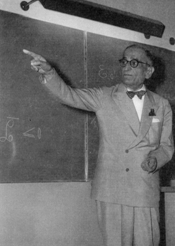
\includegraphics[width=\linewidth]{figures/Antonio_Signorini.jpg}
    \captionof*{figure}{\tiny A. Signorini}
  \end{minipage}}%
  \hfill
  \begin{minipage}[b]{0.46\textwidth}
    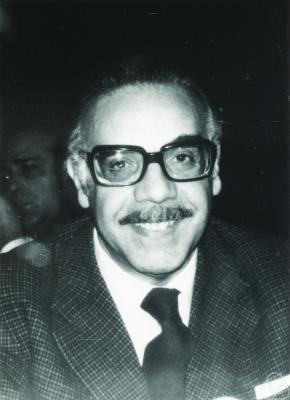
\includegraphics[width=\linewidth]{figures/Gaetano_Fichera.jpg}
    \captionof*{figure}{\tiny G. Fichera}
  \end{minipage}
\end{figure}\vspace{-8ex}
\begin{figure}
	\centering
	\begin{tikzpicture}
		\node at (-3.35,0) {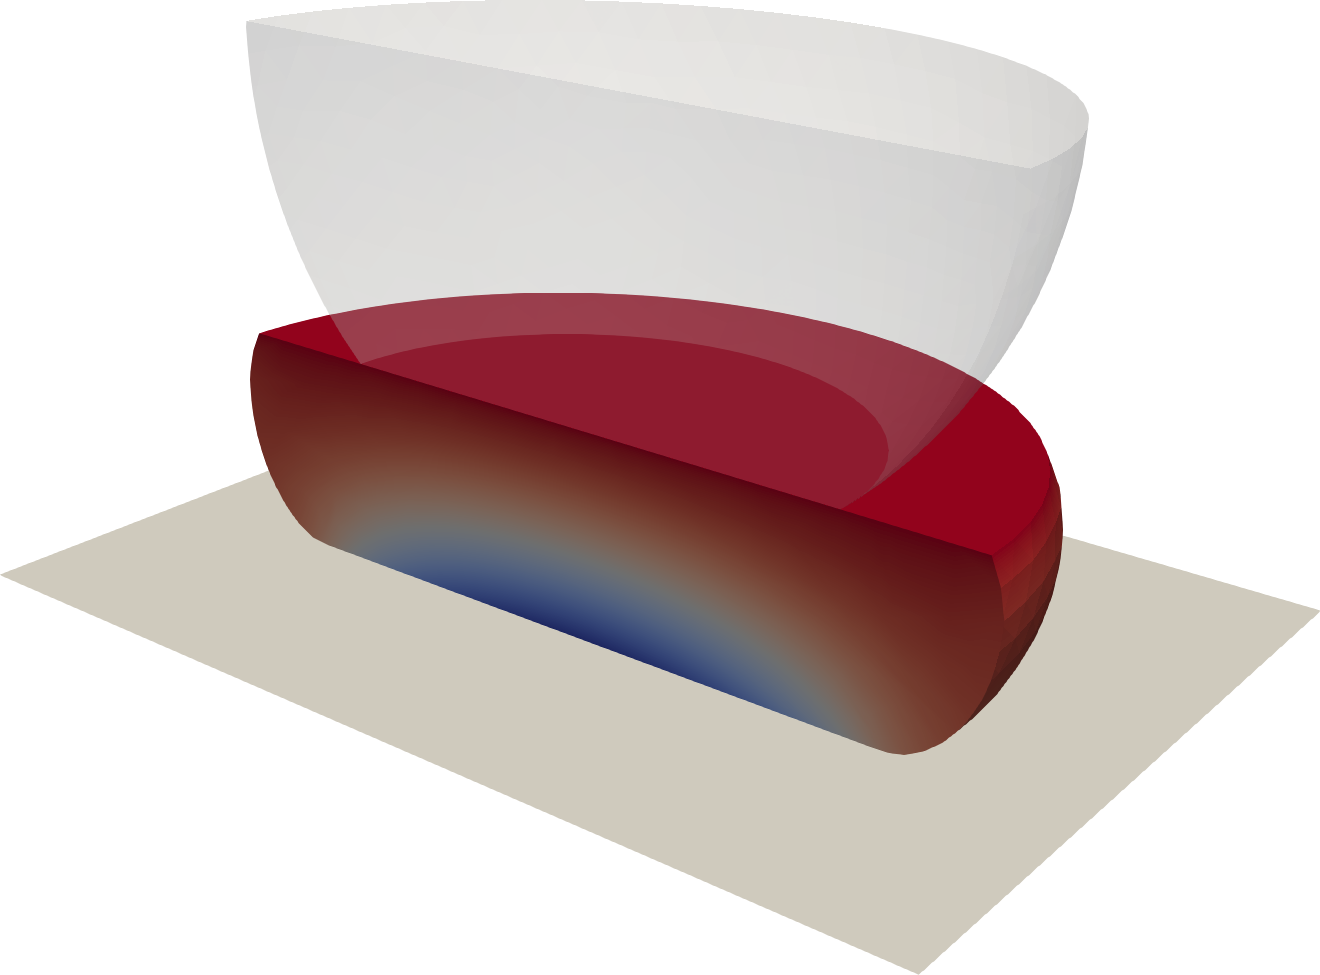
\includegraphics[height=1.25in]{figures/contact.png}};
    \end{tikzpicture}
\end{figure}
\end{minipage}
\end{frame}

\begin{frame}\frametitle{The Signorini Problem}
\begin{minipage}{0.55\linewidth}
\visible<1->{
\begin{beamercolorbox}[rounded=true, shadow=true, wd=\textwidth]{block body}
\visible<1->{State space:\vspace{-1.5ex}
\begin{equation*}
\label{eq:Signorini_V}
    V = \big\{ u \in H^1(\Omega,\mathbb{R}^3)
        \mid u = g \text{ on } \Gamma_\mathrm{D\textbf{}}
    \big\}
    \,,
\end{equation*}}\vspace{-4ex}

\visible<2->{Objective function:\vspace{-1.5ex}
\begin{equation*}
    J(u) =
    \frac{1}{2}\int_\Omega (\mathbb C \epsilon(u)) : \epsilon(u) \dd x
    -
    \int_\Omega f \cdot u \dd x
    \,,
\end{equation*}}\vspace{-2.5ex}

\visible<3->{Inequality constraints:\vspace{-1ex}
\begin{equation*}
 \alert{   K = \big\{ u \in V
        \mid u \cdot \tilde{n} \leq \phi_1 \text{ on } \Gamma_\mathrm{T}
    \big\} }
    \,.
\end{equation*}}\vspace{-4ex}
\end{beamercolorbox}
}\visible<4->{
\begin{beamercolorbox}[rounded=true, shadow=true, wd=\textwidth]{block body}\scriptsize
%Here, $\epsilon : H^1(\Omega,\mathbb{R}^3) \to L^2(\Omega,\mathbb{R}^{3\times 3}_{\mathrm{sym}})$, 
$\epsilon := (\nabla + \nabla^\top)/2$ symmetric gradient\smallskip
 
$\C \colon \mathbb{R}^{3\times 3}_{\mathrm{sym}} \to \mathbb{R}^{3\times3}_{\mathrm{sym}}$ sym.\ pos.-def.\ elasticity tensor\smallskip

$f \colon \Omega \to \mathbb{R}^3$ internal body force density\smallskip

$\phi_1 \colon \Gamma_\mathrm{T} \to \mathbb{R}_+$ gap function, $\tilde{n}$ normal to contact surface.
\end{beamercolorbox}}
\end{minipage}\hspace{4ex}
\begin{minipage}{0.3\linewidth}
 \centering
 \begin{figure}
  \centering\vspace{1ex}
  \visible<1->{\begin{minipage}[b]{0.45\textwidth}
    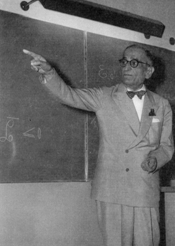
\includegraphics[width=\linewidth]{figures/Antonio_Signorini.jpg}
    \captionof*{figure}{\tiny A. Signorini}
  \end{minipage}}%
  \hfill
  \begin{minipage}[b]{0.46\textwidth}
    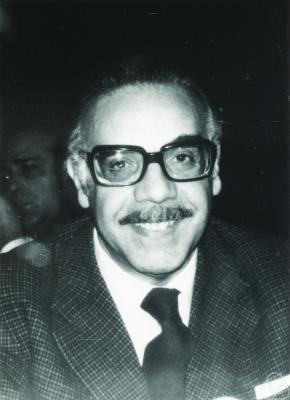
\includegraphics[width=\linewidth]{figures/Gaetano_Fichera.jpg}
    \captionof*{figure}{\tiny G. Fichera}
  \end{minipage}
\end{figure}\vspace{-8ex}
\begin{figure}
	\centering
	\begin{tikzpicture}
		\node at (-3.35,0) {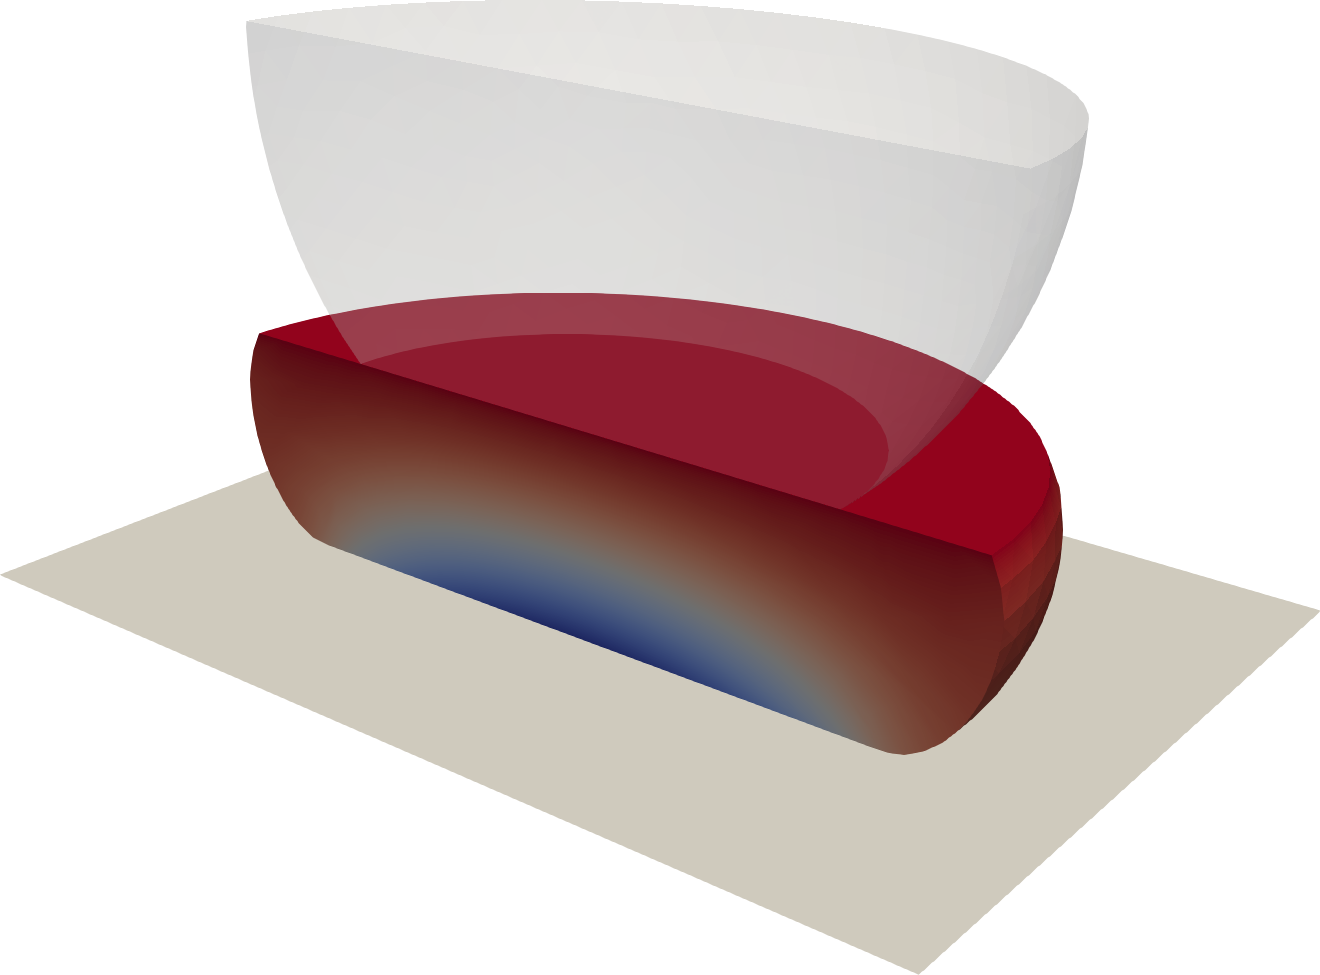
\includegraphics[height=1.25in]{figures/contact.png}};
    \end{tikzpicture}
\end{figure}
\end{minipage}
\end{frame}
%\hypertarget{example_1_alpha}{}
% \hyperlink{target_alpha}{\beamerbutton{Go to choice of $\alpha$}}
% \hyperlink{target}{\beamerbutton{Go to Finite Element Spaces}}
%  \hyperlink{target_alg}{\beamerbutton{Go to Algorithm and Convergence}}


\begin{frame}\frametitle{Gradient Constraints}
\begin{minipage}{0.55\linewidth}
\visible<1->{
\begin{beamercolorbox}[rounded=true, shadow=true, wd=\textwidth]{block body}
\footnotesize}\visible<1->{Often arise in \alert{Quasi-Variational Inequalities} (QVIs).\\
 
 }\visible<2->{
Major contributions by L. Prigozhin (modeling), J.F. Rodrigues (analysis), M. Hinterm\"uller \& C.N. Rautenberg (algorithms), and many others.\\
 
 }\visible<3->{
Diverse applications: 
\begin{itemize}
\item Elastic-plastic torsion problem
\item Sandpile growth
\item Magnetization in type-II superconductors
\item Hydrology 
\item Simplified stress constraints.
\end{itemize}}
\end{beamercolorbox}

%\visible<2->{
%\begin{beamercolorbox}[rounded=true, shadow=true, wd=\textwidth]{block body}
%\visible<2->{$\Omega \subset \mathbb{R}^3$, $\Gamma$ split into two disjoint subsets.}
%\visible<2->{$\Gamma = \overline{ \Gamma_\mathrm{D} \cup \Gamma_\mathrm{T} }$ with\\
%$\Gamma_D$ for \textbf{d}isplacement\\
%$\Gamma_{T}$ for \textbf{t}raction boundary conditions.}
%\end{beamercolorbox}}
\end{minipage}\hspace{4ex}
\begin{minipage}{0.3\linewidth}
 \centering
 \begin{figure}
  \centering\vspace{1ex}
  \visible<1->{\begin{minipage}[b]{0.38\textwidth}
    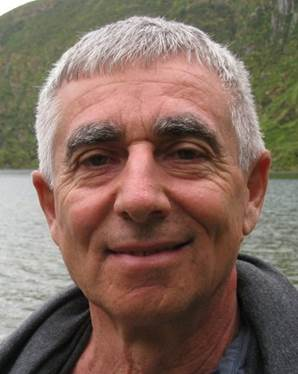
\includegraphics[width=\linewidth]{figures/Prigozhin.jpg}
    \captionof*{figure}{\tiny L. Prigozhin}
  \end{minipage}}%
  \hfill
  \begin{minipage}[b]{0.46\textwidth}
    \includegraphics[width=\linewidth]{figures/Rodrigues.jpg}
    \captionof*{figure}{\tiny J.F. Rodrigues}
  \end{minipage}
\end{figure}
 \begin{minipage}[b]{0.5\textwidth}
    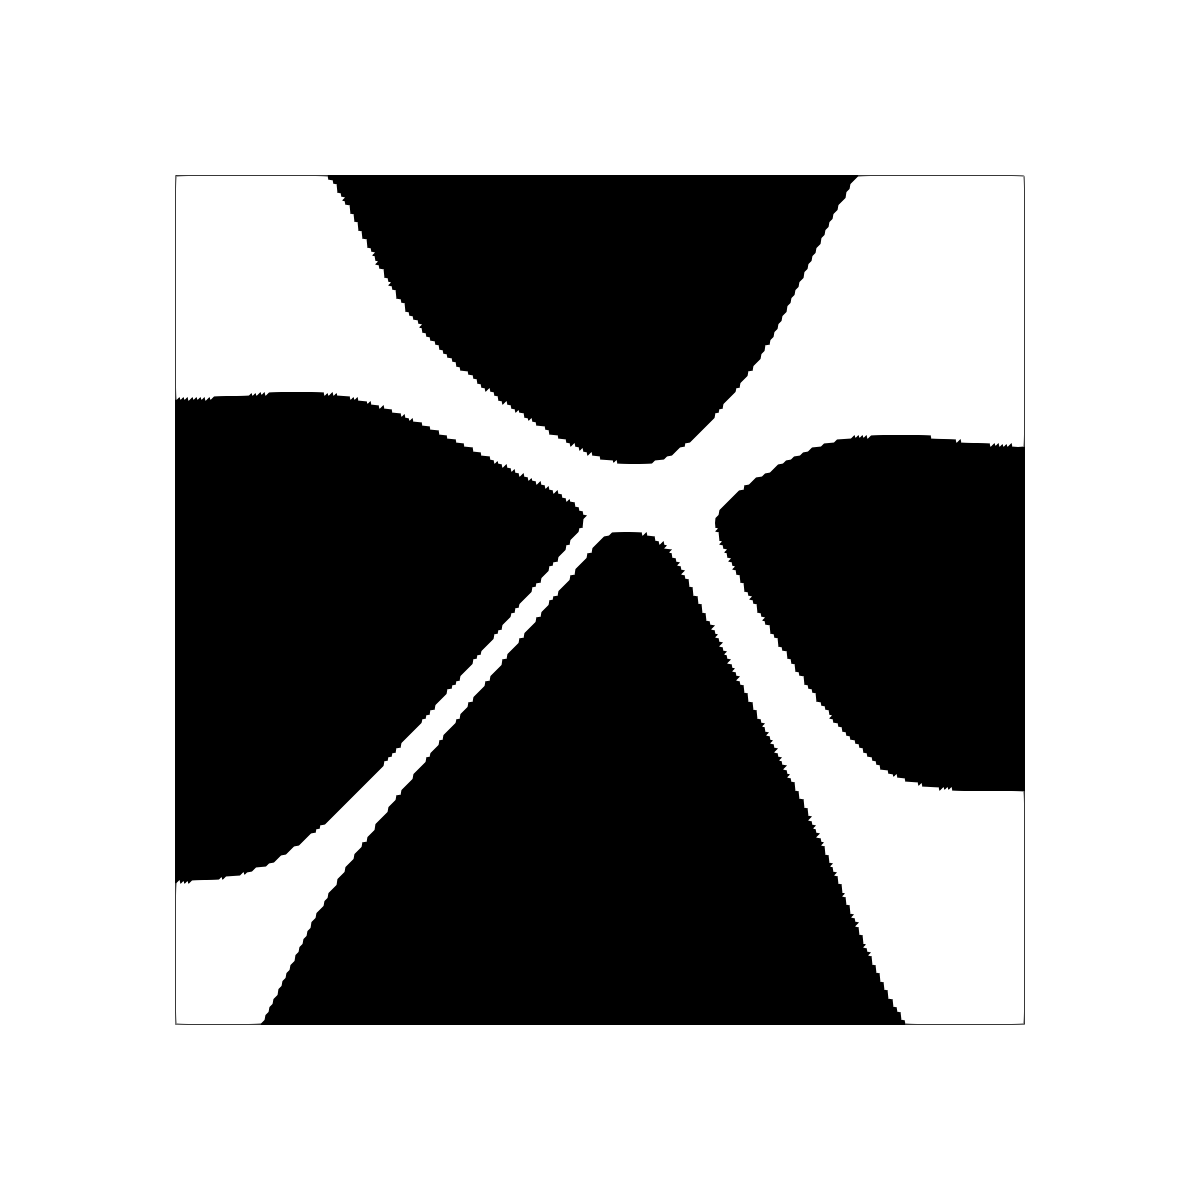
\includegraphics[width=\linewidth]{figures/global_feasible_active_set.png}
    \captionof*{figure}{\tiny Black: $|\nabla u| = \phi$.}
  \end{minipage}%
%  \hfill
%  \begin{minipage}[b]{0.6\textwidth}
    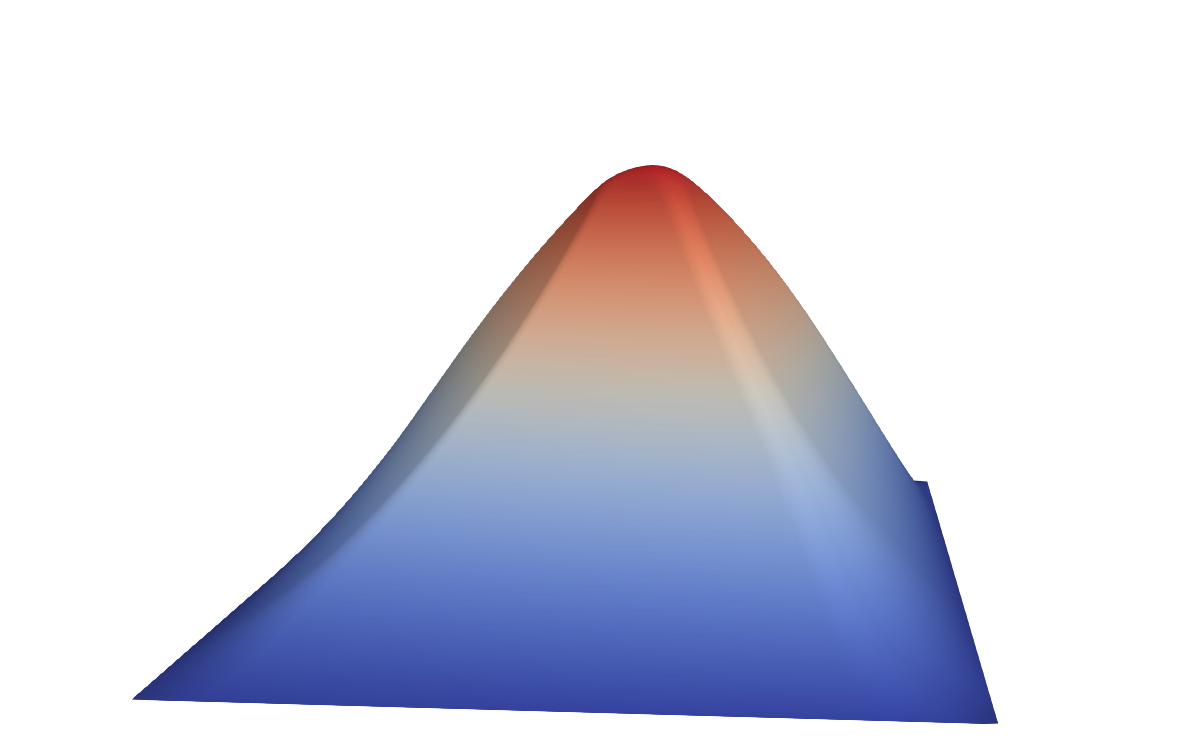
\includegraphics[width=0.8\linewidth]{figures/gradient_constraint_u.png}
%    \captionof*{figure}{\tiny State $u$}
%  \end{minipage}
%\begin{figure}
%	\centering
%	\begin{tikzpicture}
%		\node at (-5,0) {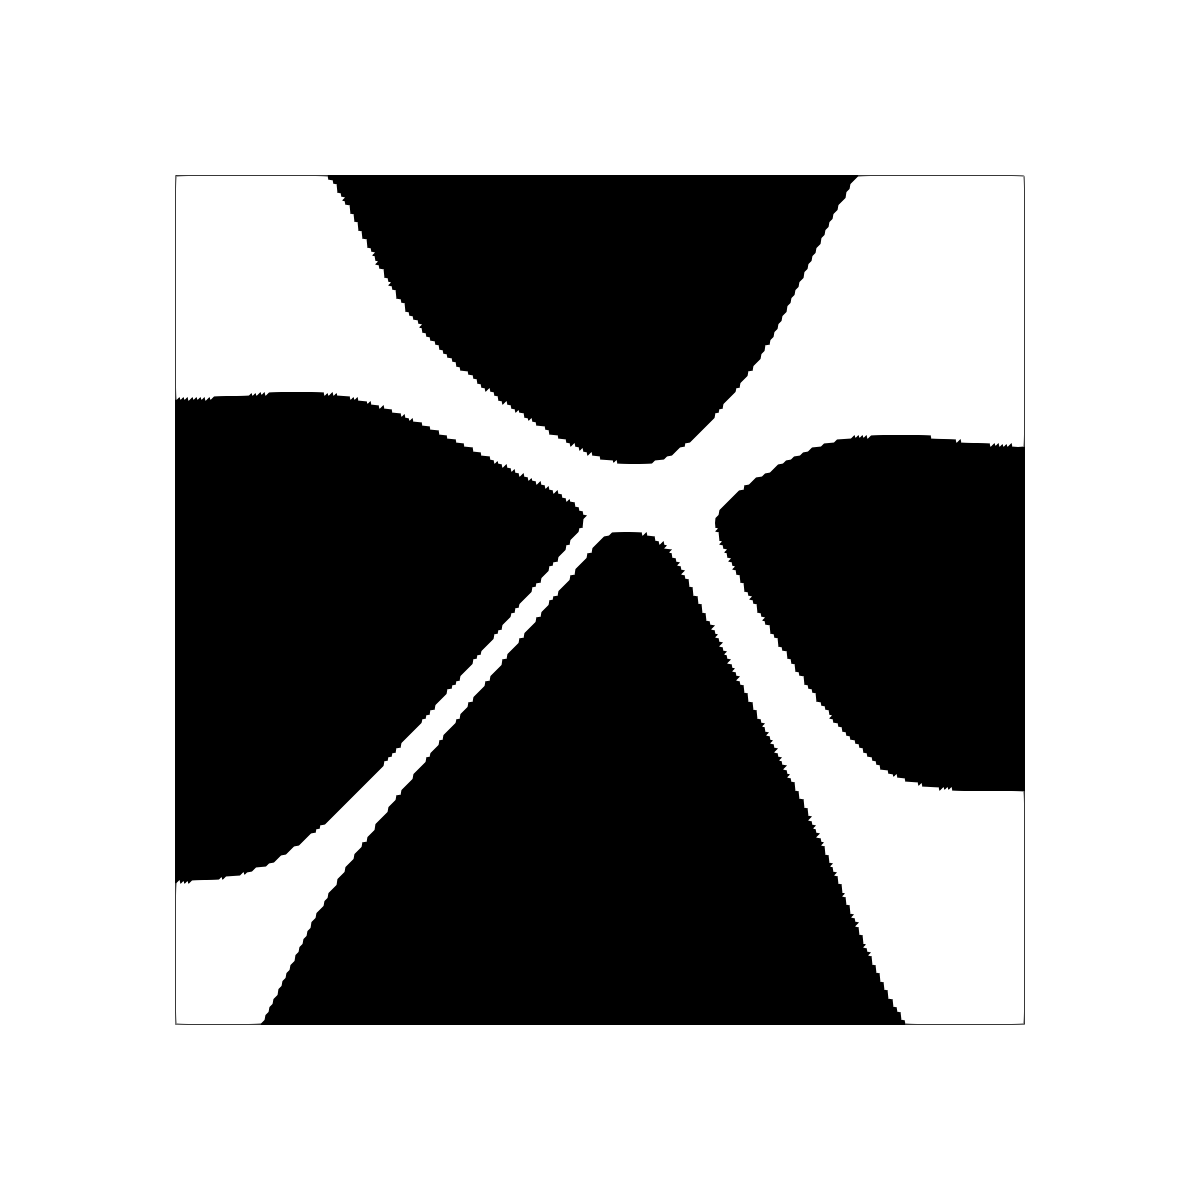
\includegraphics[height=1in]{figures/global_feasible_active_set.png}};\hspace{10ex}
%    \end{tikzpicture}\vspace{-8ex}
%	\begin{tikzpicture}
%		\node at (-2,-1) {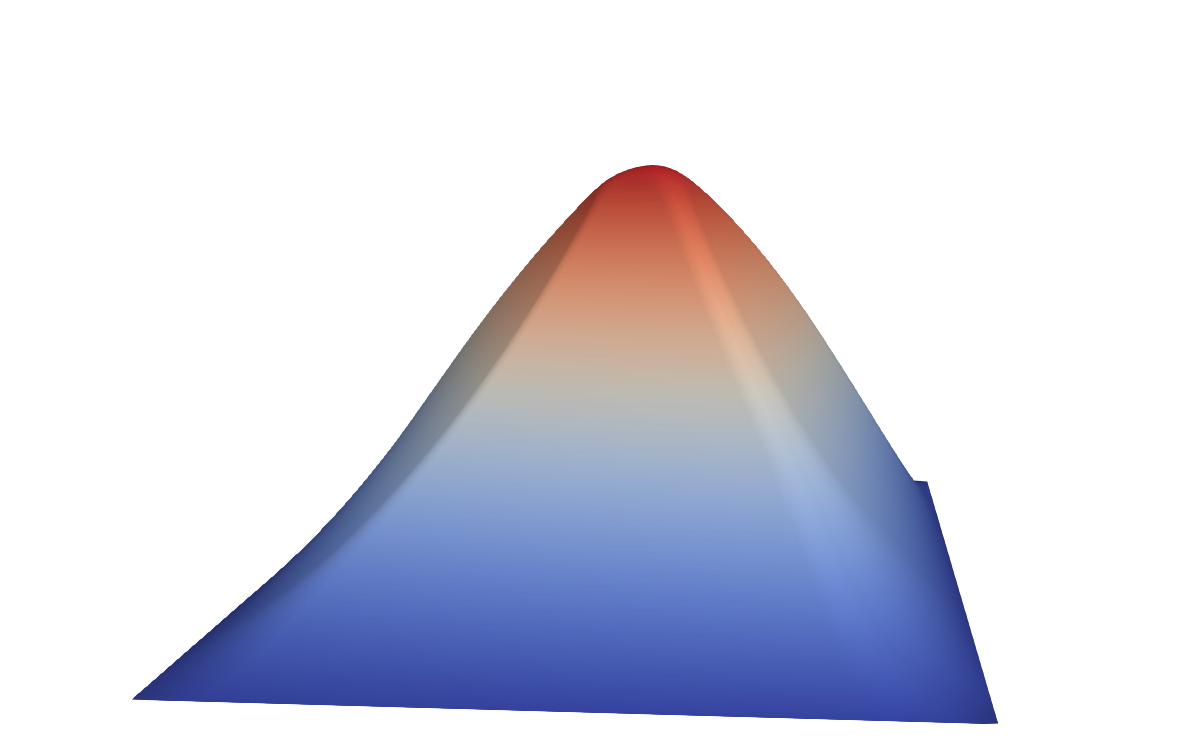
\includegraphics[height=1.25in]{figures/gradient_constraint_u.png}};
%    \end{tikzpicture}
%%\end{figure}
%  \end{minipage}
\end{minipage}
\end{frame}

\begin{frame}\frametitle{Gradient Constraints}
\begin{minipage}{0.55\linewidth}
\visible<1->{
\begin{beamercolorbox}[rounded=true, shadow=true, wd=\textwidth]{block body}
\footnotesize\visible<1->{Domain: $\Omega \subset \mathbb{R}^n$ open, bounded, Lipschitz\\

}\visible<2->{
State space: $V := W^{1,p}_0(\Omega)$ with $p \ge 2$\\

}\visible<3->{
Objective function:
 \begin{equation*}\label{eq:grad-ob}
     J(u) :=  \frac{1}{p} \int_{\Omega}|\nabla u|^p - f u \dd x
 \end{equation*}
Forcing term $f \in L^2(\Omega)$\medskip

}\visible<4->{
\alert{Inequality constraints:
\begin{equation}\label{eq:grad-constr}
K = \{ u \in H^1_0(\Omega) \mid |\nabla u| \le \phi \text{ a.e.\ in } \Omega \}\,.
\end{equation}
}
$\phi \in L^{\infty}(\Omega)$ : $\phi \ge \epsilon$ a.e.\ for constant $\epsilon > 0$.
}


\end{beamercolorbox}
}
%\visible<2->{
%\begin{beamercolorbox}[rounded=true, shadow=true, wd=\textwidth]{block body}
%\visible<2->{$\Omega \subset \mathbb{R}^3$, $\Gamma$ split into two disjoint subsets.}
%\visible<2->{$\Gamma = \overline{ \Gamma_\mathrm{D} \cup \Gamma_\mathrm{T} }$ with\\
%$\Gamma_D$ for \textbf{d}isplacement\\
%$\Gamma_{T}$ for \textbf{t}raction boundary conditions.}
%\end{beamercolorbox}}
\end{minipage}\hspace{4ex}
\begin{minipage}{0.3\linewidth}
 \centering
 \begin{figure}
  \centering\vspace{1ex}
  \visible<1->{\begin{minipage}[b]{0.38\textwidth}
    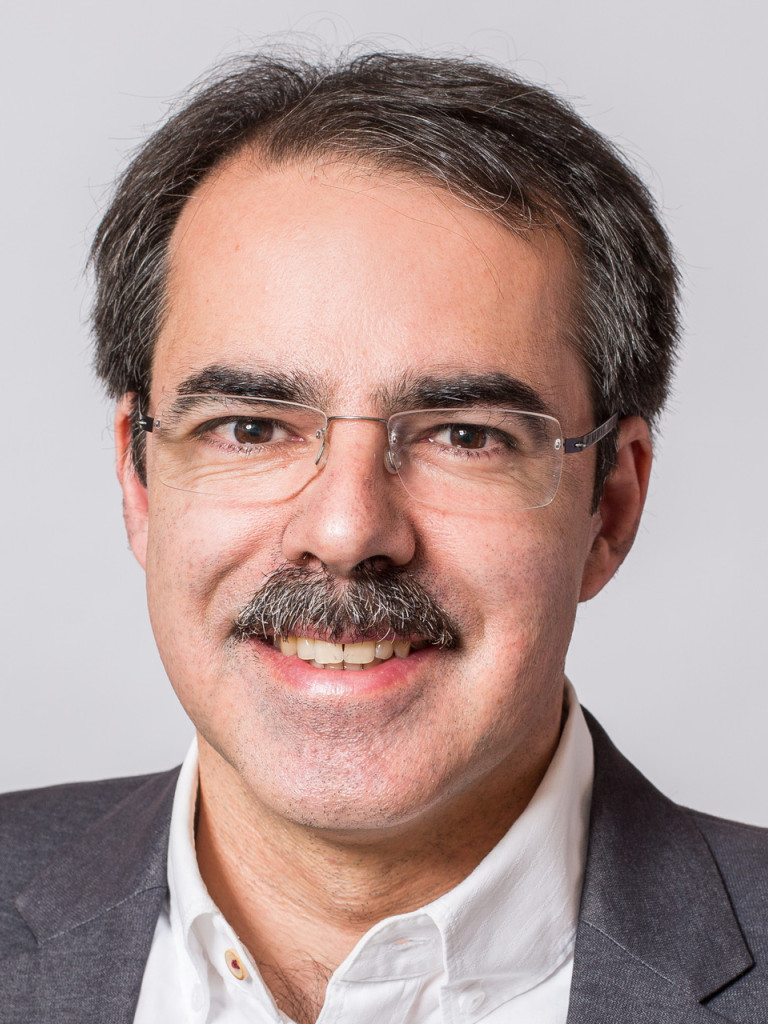
\includegraphics[width=\linewidth]{figures/hintermueller.jpg}
    \captionof*{figure}{\tiny M. Hinterm\"uller}
  \end{minipage}}%
  \hfill
  \begin{minipage}[b]{0.46\textwidth}
    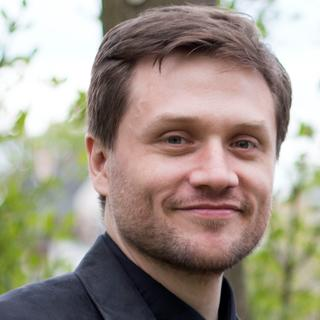
\includegraphics[width=\linewidth]{figures/rautenberg.jpg}
    \captionof*{figure}{\tiny C.N. Rautenberg}
  \end{minipage}
\end{figure}
 \begin{minipage}[b]{0.5\textwidth}
    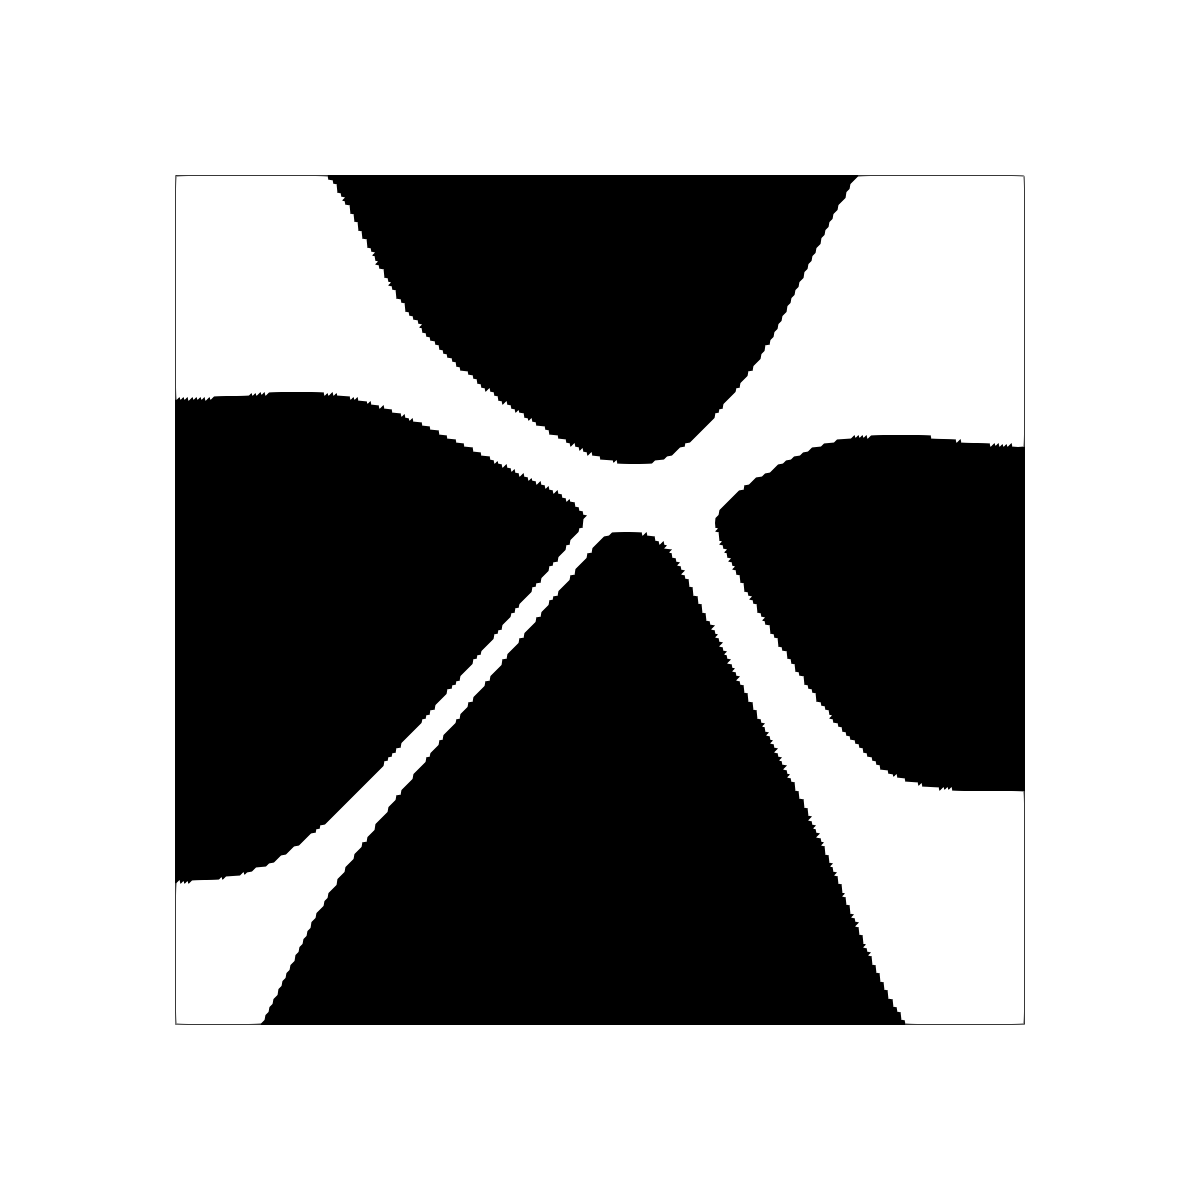
\includegraphics[width=\linewidth]{figures/global_feasible_active_set.png}
    \captionof*{figure}{\tiny Black: $|\nabla u| = \phi$.}
  \end{minipage}%
%  \hfill
%  \begin{minipage}[b]{0.6\textwidth}
    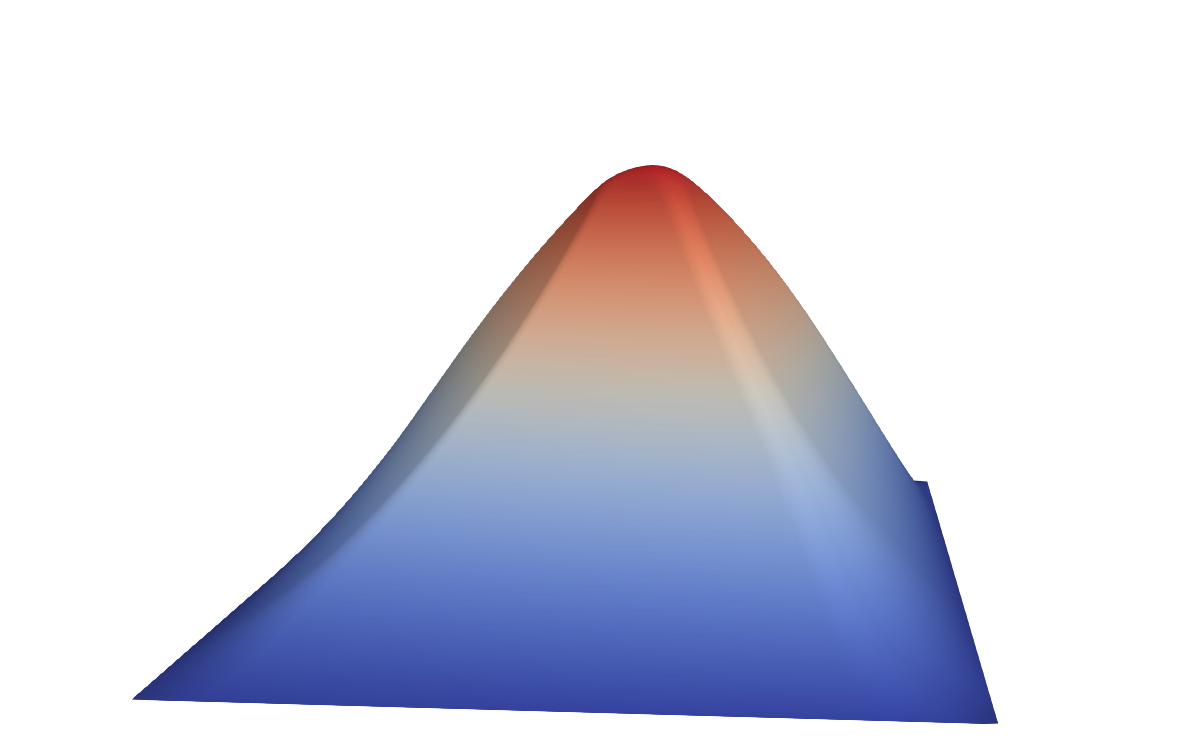
\includegraphics[width=0.8\linewidth]{figures/gradient_constraint_u.png}
%    \captionof*{figure}{\tiny \hspace{28ex} State $u$ for $p=2$}
%  \end{minipage}
%\begin{figure}
%	\centering
%	\begin{tikzpicture}
%		\node at (-5,0) {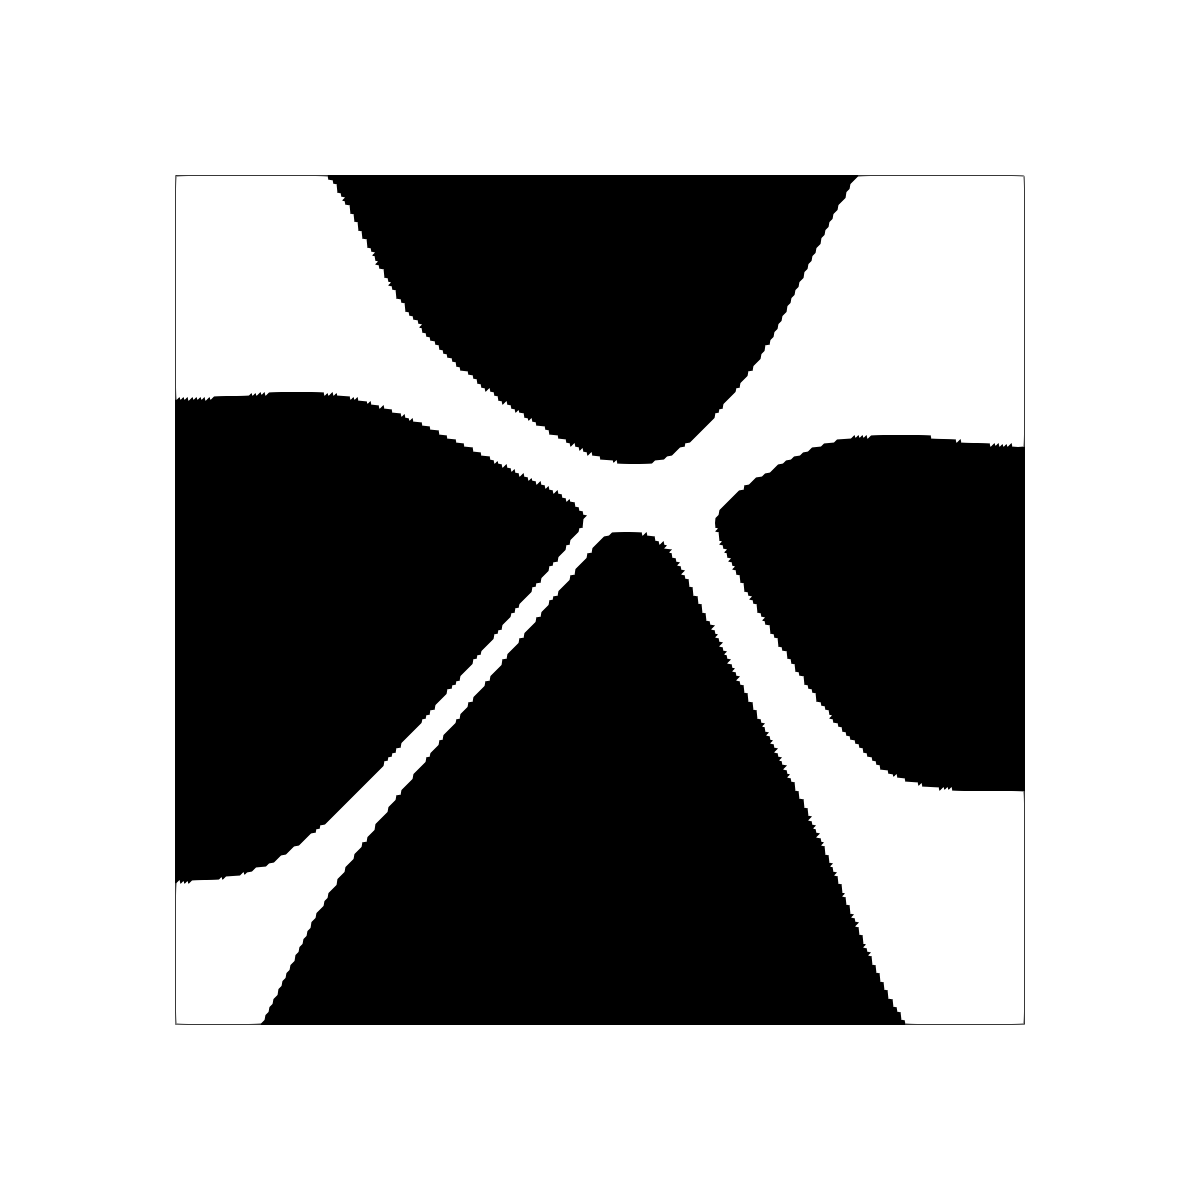
\includegraphics[height=1in]{figures/global_feasible_active_set.png}};\hspace{10ex}
%    \end{tikzpicture}\vspace{-8ex}
%	\begin{tikzpicture}
%		\node at (-2,-1) {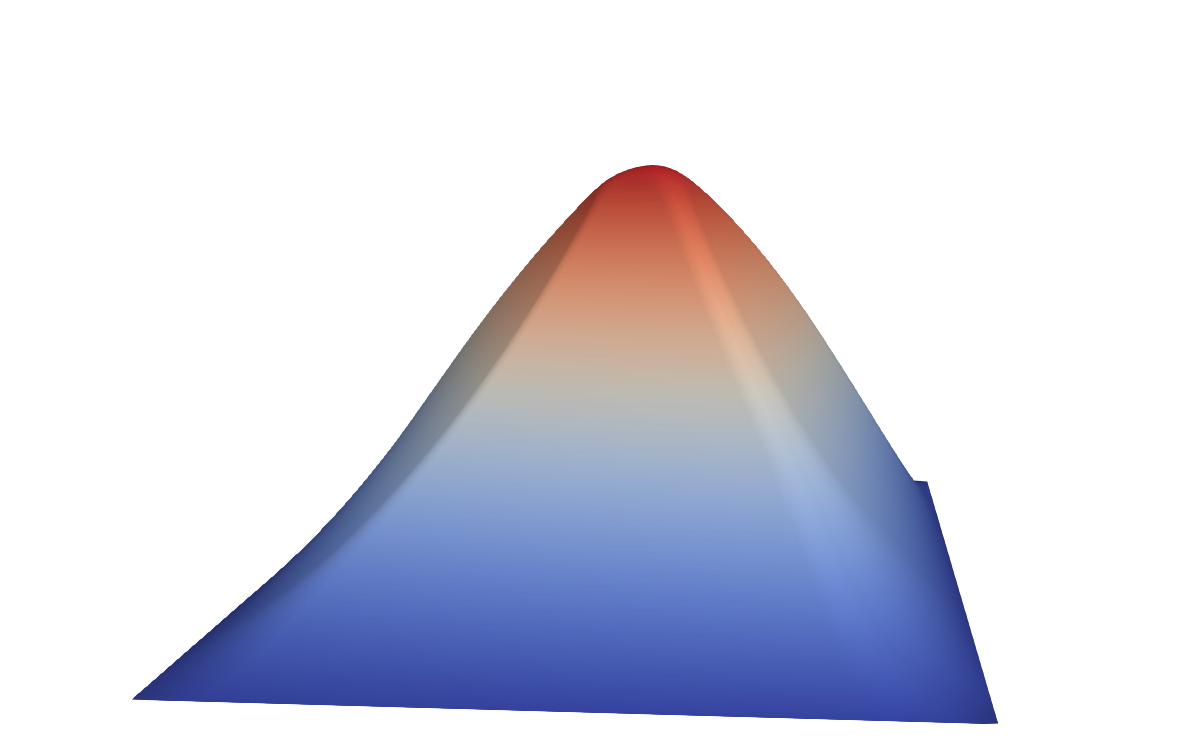
\includegraphics[height=1.25in]{figures/gradient_constraint_u.png}};
%    \end{tikzpicture}
%%\end{figure}
%  \end{minipage}
\end{minipage}
\end{frame}

\begin{frame}{Further Examples}
\begin{figure}
  \centering
  \begin{subfigure}[b]{0.19\textwidth}
    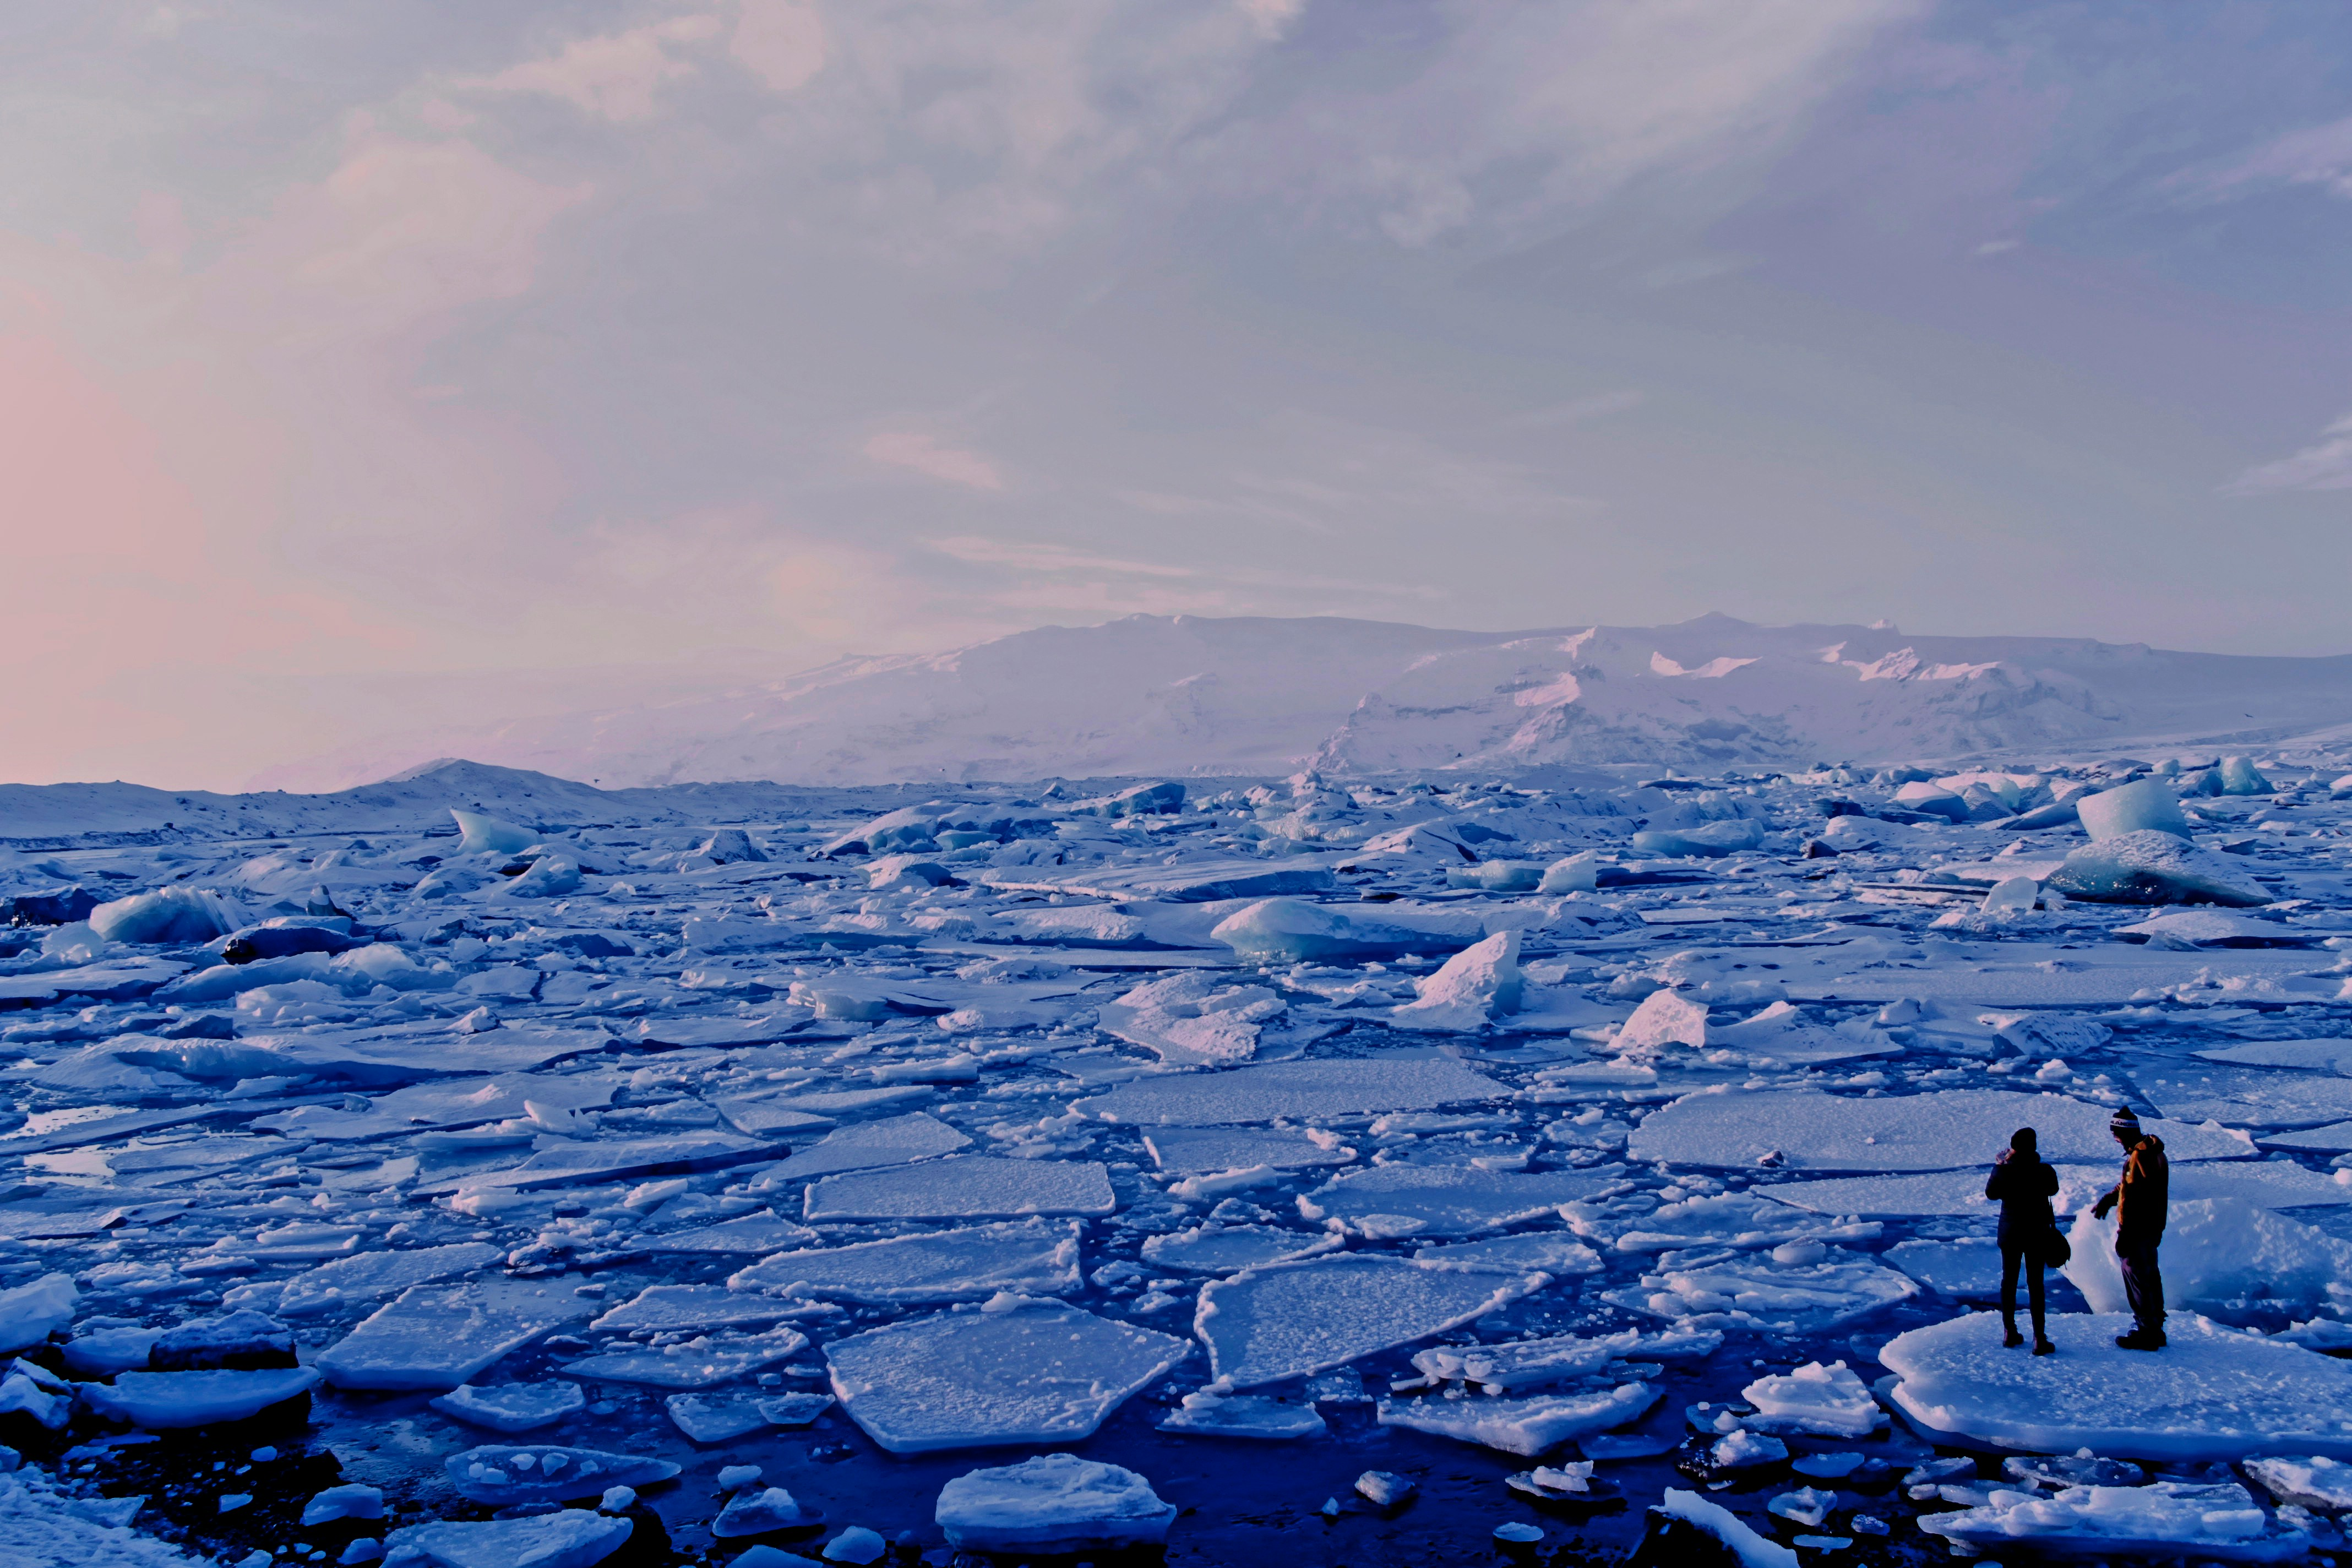
\includegraphics[width=\linewidth]{figures/ice.jpg}
    \caption{Stefan Problem}
  \end{subfigure}
  \hfill
  \begin{subfigure}[b]{0.19\textwidth}
    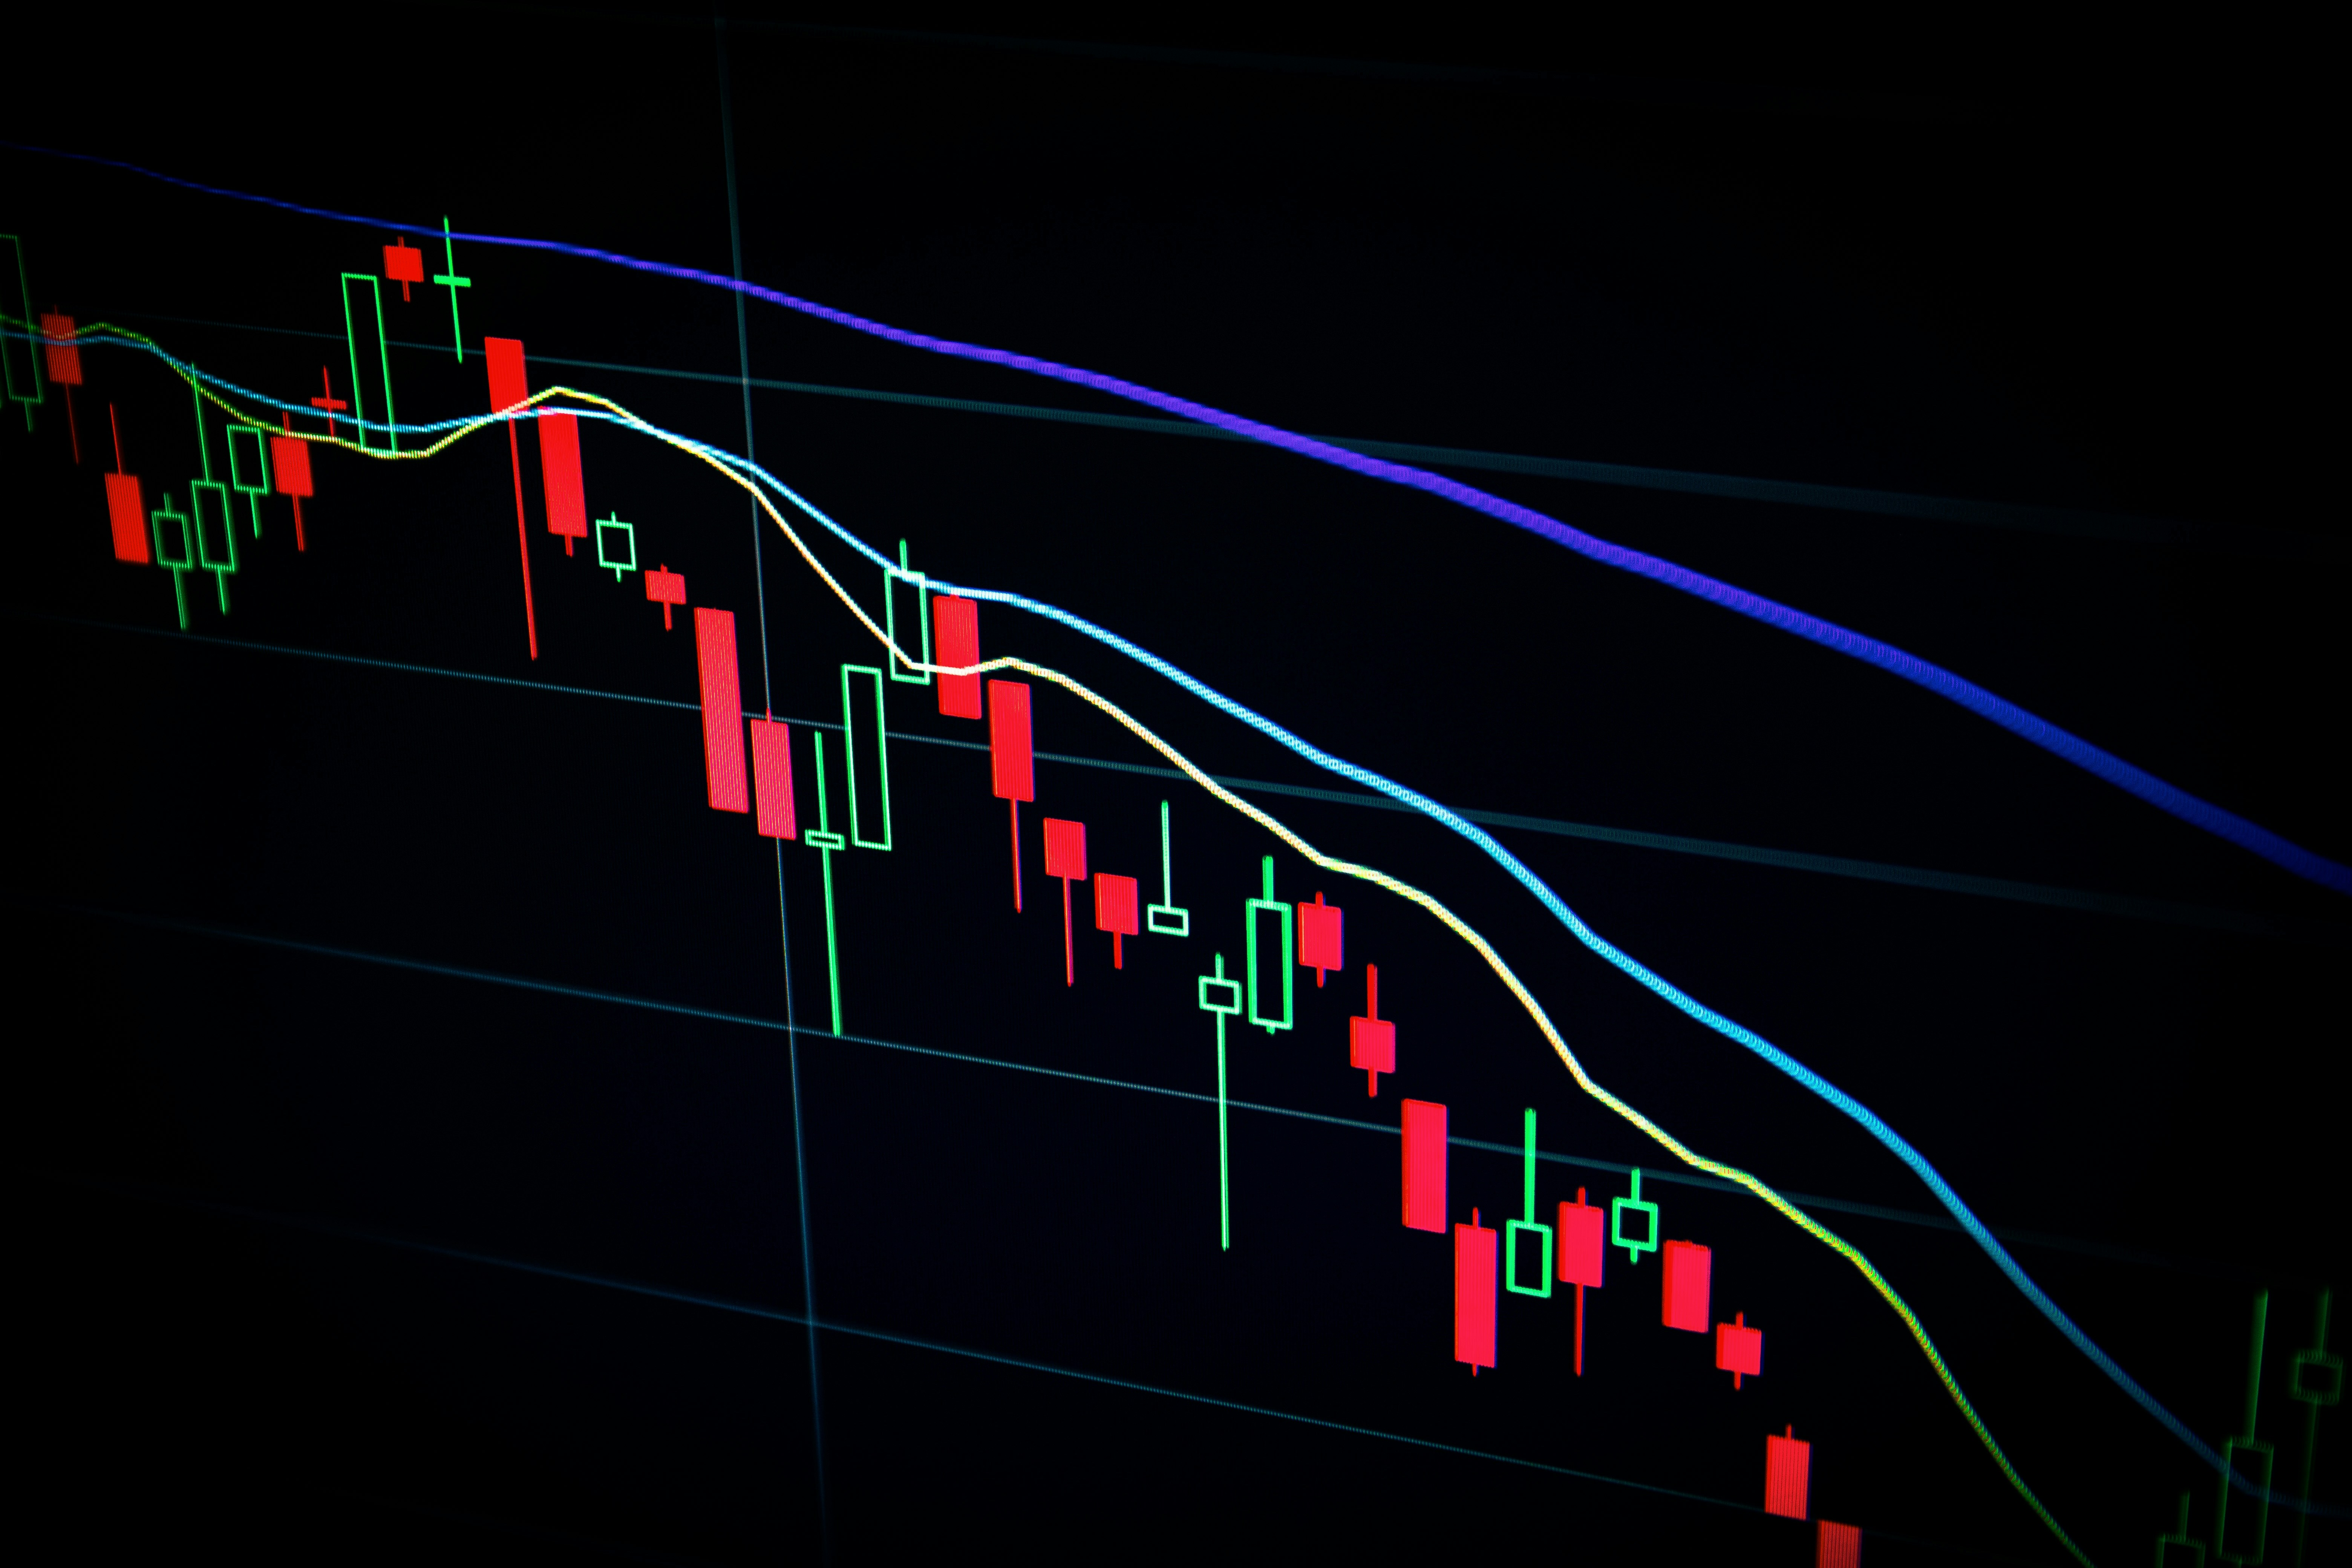
\includegraphics[width=\linewidth]{figures/stocks.jpg}
    \caption{Option Pricing}
  \end{subfigure}
  \hfill
  \begin{subfigure}[b]{0.19\textwidth}
    \includegraphics[width=\linewidth]{figures/water-oil-2.jpg}
    \caption{Phase Transition}
  \end{subfigure}\\
%  \hfill
  \begin{subfigure}[b]{0.19\textwidth}
    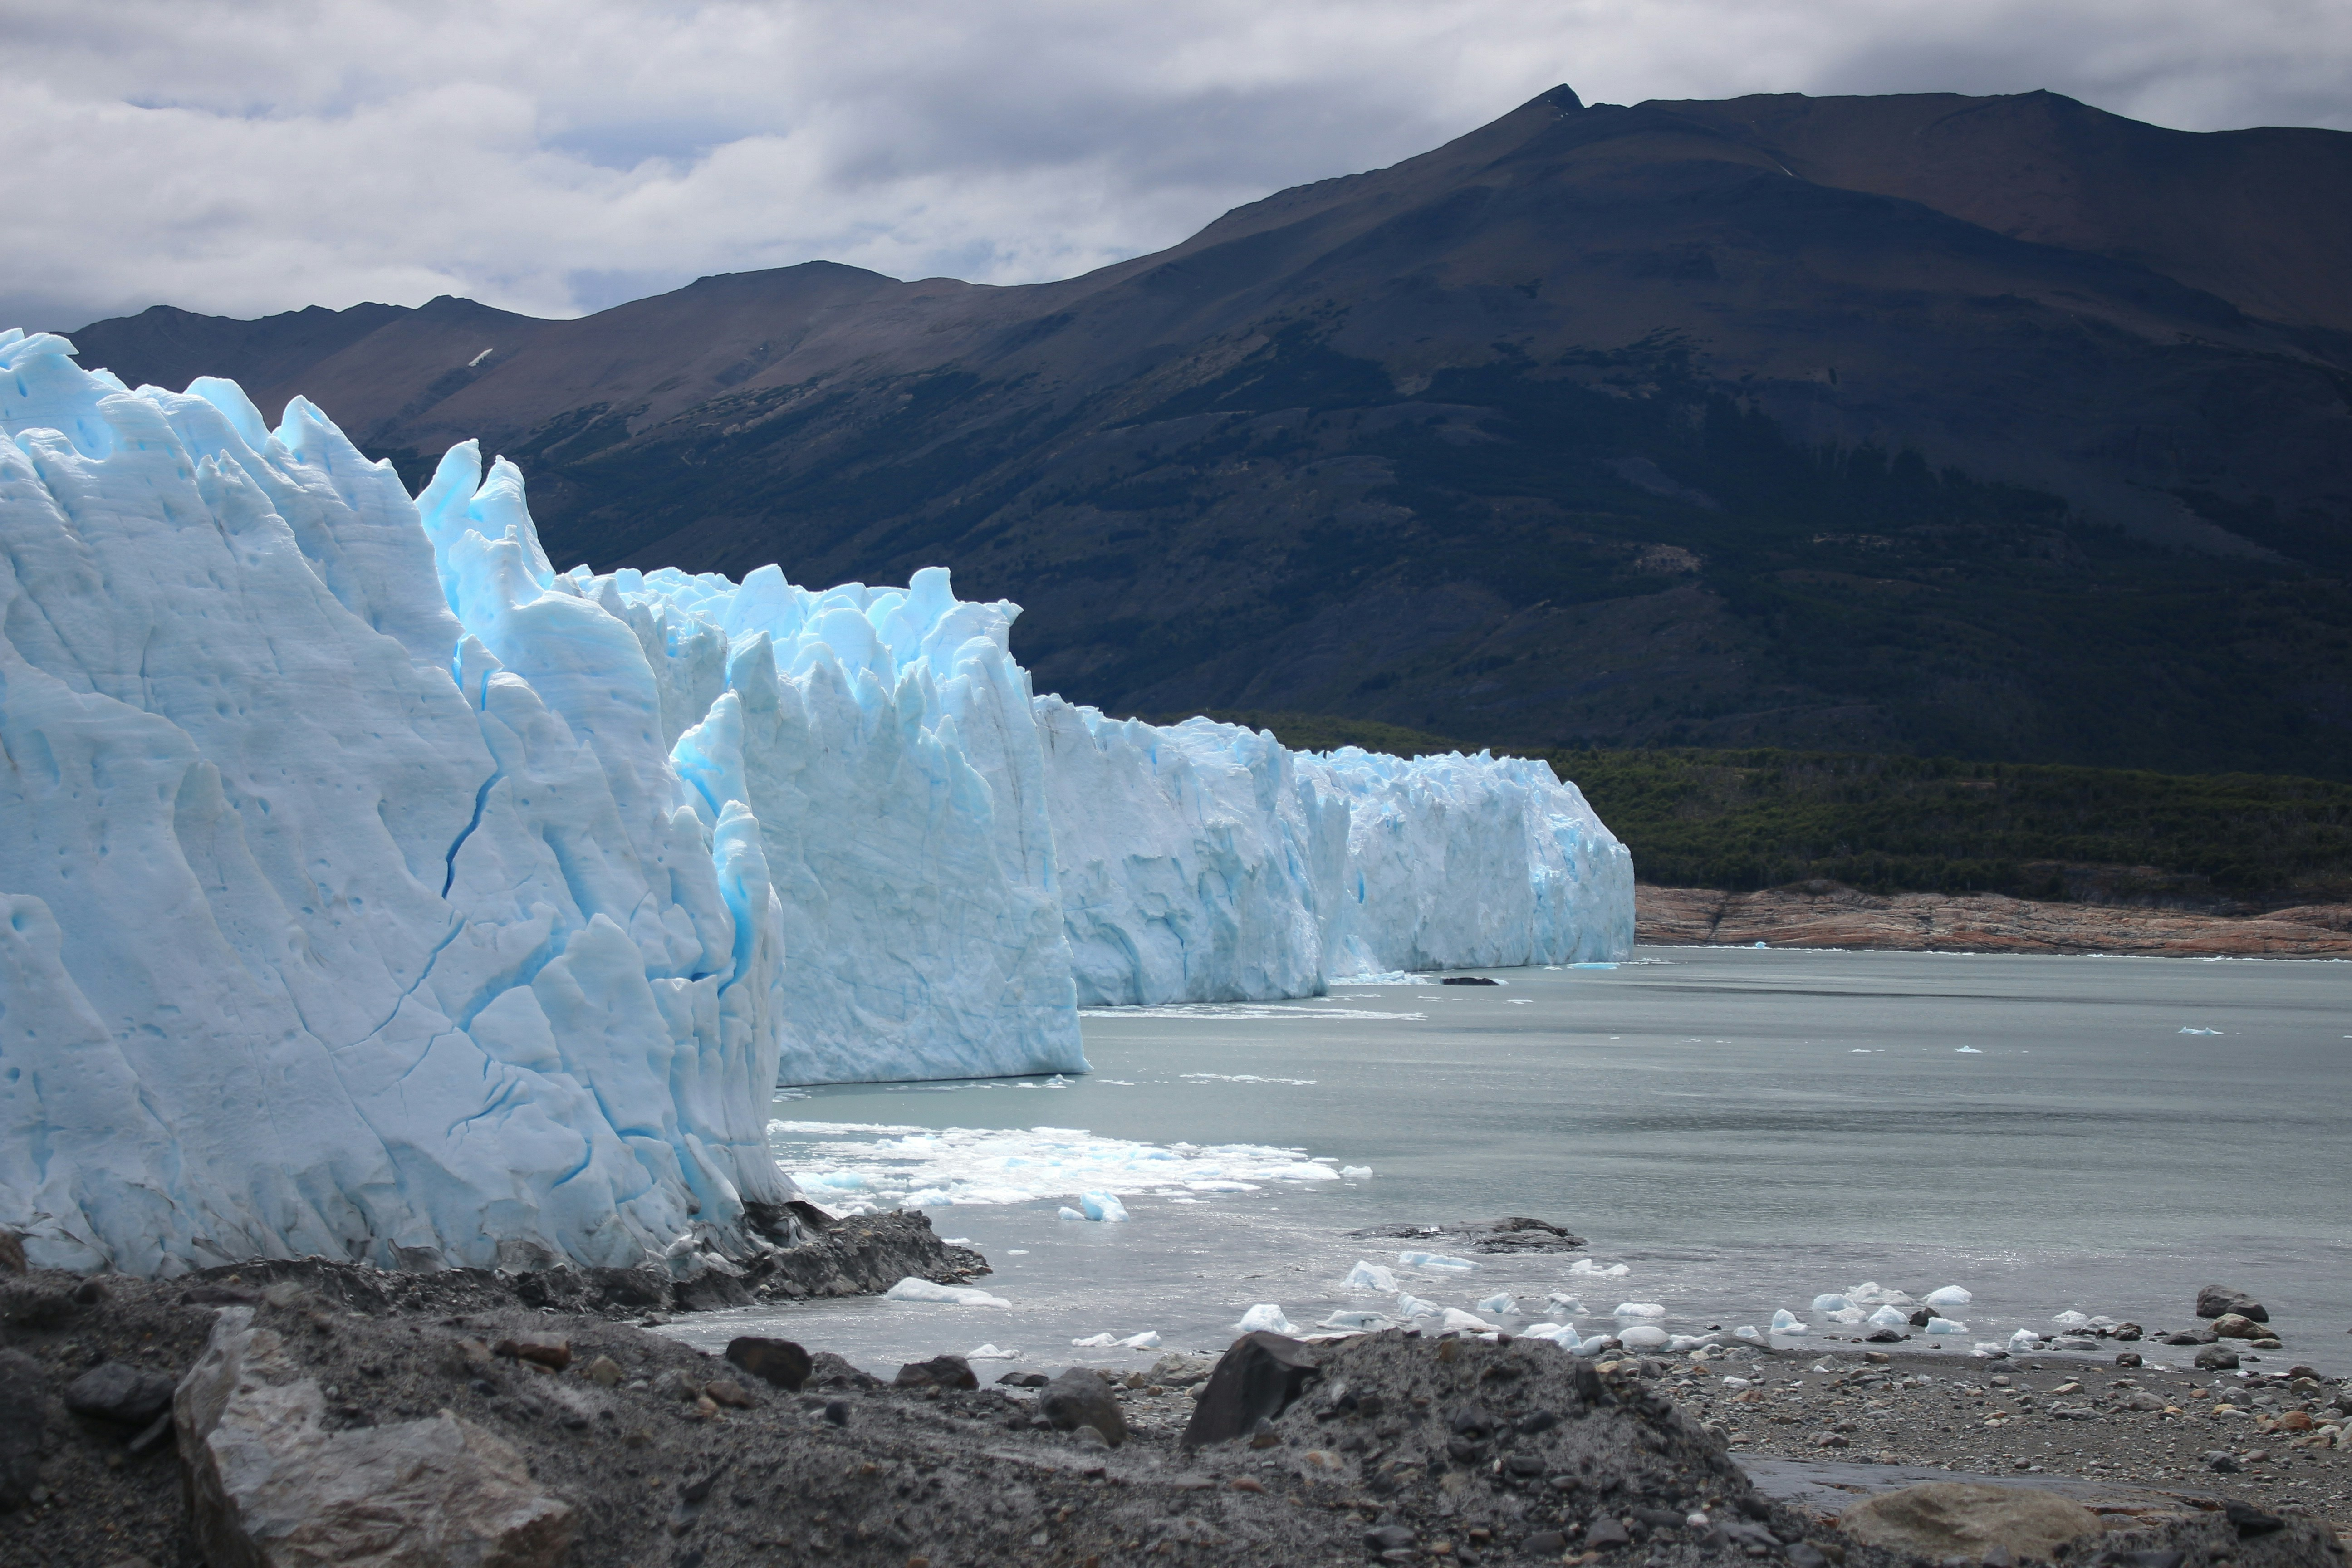
\includegraphics[width=\linewidth]{figures/glacier.jpg}
    \caption{Ice Sheet Models}
  \end{subfigure}
\hspace{7em}	
%  \hfill
  \begin{subfigure}[b]{0.19\textwidth}
    \includegraphics[width=\linewidth]{figures/rivers.jpg}
    \caption{Diffusive Waves}
  \end{subfigure}
\end{figure}
 \visible<1->{\begin{beamercolorbox}[rounded=true, shadow=true, wd=\textwidth]{block title}
 \centering Each one of these applications can be formulated as a variational inequality with nontrivial pointwise inequality constraints on the state!
 \end{beamercolorbox}
 }
\end{frame}

%\section{Examples}\label{sec:examples}
%\begin{frame}{Examples of Variational Inequalities}
%    \begin{enumerate}
%%        \item Signorini problem
%%        \item Stefan problem
%%        \item Black-Scholes
%%        \item Multiphase phase transition
%%        \item Elastoplastic torsion
%%        \item Ice sheet
%        \item Diffusive wave equation
%    \end{enumerate}
%\end{frame}

%\begin{frame}{Elliptic Variational Inequalities}
%        \begin{enumerate}
%        \item A slight twist on Dirichlet's principle
%            \begin{enumerate}
%                \item Conic constraint ($u \ge 0$)
%                \item Follow Dirichlet above for derivation
%            \end{enumerate}
%        \item A second variational inequality: An obstacle problem
%        \item A brief history of variational inequalities (of the first kind)
%        \item The Lions-Stampacchia theorem
%        \item Mignot's theorem
%            \begin{enumerate}
%                \item 
%            \end{enumerate}
%    \end{enumerate}
%\end{frame}

\begin{frame}\frametitle{The Obstacle Problem}
\only<1-3>{
\begin{minipage}{0.45\linewidth}
\begin{beamercolorbox}[rounded=true, shadow=true, wd=\textwidth]{block body}
 \visible<1->{A deceptively simple twist on Dirichlet's principle...\medskip
 
 }\visible<2->{
 We seek a minimizer $u$ of the total energy functional:
 \begin{equation*}
 	E(v)
 	=
 	\frac{1}{2}
 	\int_\Omega |\nabla v|^2 \dd x
 	-
 	\int_\Omega f v\dd x
 	\,,
 \end{equation*}
 
  }\visible<3->{
 over the \textbf{closed convex set} defined by  
 \[
 K = \{ v \in H^1(\Omega) \mid  v \ge \varphi \text{~a.e. }  u|_{\Gamma} = g \}
 \] 
 with $\varphi \in H^1(\Omega)$, $(\varphi - g)|_{\Gamma} \ge 0$.
} 
\end{beamercolorbox}
\end{minipage}}%
\only<4->{
\begin{minipage}{0.45\linewidth}
\begin{beamercolorbox}[rounded=true, shadow=true, wd=\textwidth]{block title}
 \visible<1->{A deceptively simple twist on Dirichlet's principle...\medskip
 
 }\visible<2->{
 We seek a minimizer $u$ of the total energy functional:
 \begin{equation*}
 	E(v)
 	=
 	\frac{1}{2}
 	\int_\Omega |\nabla v|^2 \dd x
 	-
 	\int_\Omega f v\dd x
 	\,,
 \end{equation*}
 
  }\visible<3->{
 over the \textbf{closed convex set} defined by  
 \[
 K = \{ v \in H^1(\Omega) \mid  v \ge \varphi \text{~a.e. }  u|_{\Gamma} = g \}
 \] 
 with $\varphi \in H^1(\Omega)$, $(g - \varphi)|_{\Gamma} \ge 0$.
} 
\end{beamercolorbox}
\end{minipage}}%
\only<4->{%
\begin{minipage}{0.55\linewidth}
%\hspace{-4ex}
\begin{beamercolorbox}[rounded=true, shadow=true, wd=\textwidth]{block body}
Existence of solutions:
\begin{itemize}
\item \visible<5->{The analysis follows Dirichlet's principle.}
\item \visible<6->{\alert{New}: We must view $E : K \subsetneq H^1(\Omega) \to \overline{\mathbb R}$}
\item \visible<7->{Is $K$ weakly sequentially compact? \alert{No.}}
\item \visible<8->{We  \alert{can}, however, show that $K \cap N_0$ is!}
\end{itemize}
\end{beamercolorbox}
\end{minipage}}
\end{frame}

\begin{frame}\frametitle{Direct Method: Extra Step}
\begin{beamercolorbox}[rounded=true, shadow=true, wd=\textwidth]{block body}\scriptsize
\visible<1->{$K \ne \emptyset$ : Construct a feasible point using Dirichlet's principle and the Maximum Principle.\bigskip

}\visible<2->{$K$ is convex: $v,w \in K$, $\lambda \in [0,1]$ $\Rightarrow$ $\lambda v + (1-\lambda) w \ge \lambda \varphi + (1-\lambda) \varphi = \varphi$, same as before for boundary data.\bigskip

}\visible<3->{$K$ is closed:  \visible<4->{Take $\left\{v_k\right\} \subset K$ such that $v_k \to v$ (strongly) in $H^1(\Omega)$. }
\begin{itemize}
\item \visible<5->{Clearly, $v_k-\varphi \to v-\varphi$ (strongly) in $L^2(\Omega)$.} 
\item \visible<6->{For any $w \in L^2(\Omega)$ : $w \ge 0$, we have $(v_k-\varphi,w) \ge 0$. Hence, $(v-\varphi,w) \ge 0$.}
\item \visible<7->{Since $w$ is arbitrary, $v \ge \phi$ a.e.\ in $\Omega$.}
%\item \visible<5->{$H^1(\Omega) \hookrightarrow L^1(\Omega)$ continuously, hence $v_k \to v$ (strongly) in $L^1(\Omega)$.} 
%\item \visible<6->{$L^1(\Omega)$ convergence implies  $\exists \left\{v_{k_l}\right\} \subset \left\{v_k\right\}$ such that $v_{k_l} \to v$ pointwise a.e.}
%\item \visible<7->{For all $k$: $v_{k} \ge \varphi$ a.e.\ (by definition), clearly for $k_l$ as well. Hence, $v \ge \varphi$.}
\item \visible<8->{The trace is continuous, hence $g = v_{k}|_{\Gamma} \to v|_{\Gamma} = g$.}
\end{itemize}}\bigskip

\visible<9->{$K$ is \alert{weakly closed}: Closed convex sets in locally convex TVS are the intersections of all closed half spaces containing them, thus weakly closed ($\Rightarrow$ \alert{weakly sequentially closed}).\bigskip

}\visible<10->{
If $\{v_k\} \subset K \cap N_0$ is a minimizing sequence, then its weak accumulation points lie in $K$!
}
\end{beamercolorbox}
\end{frame}

\begin{frame}\frametitle{The Obstacle Problem}
\begin{beamercolorbox}[rounded=true, shadow=true, wd=\textwidth]{block body}
Same arguments as in DP lead to a variational inequality as an optimality condition:\medskip

Find $u \in K$ such that
 \[
 (\nabla u, \nabla [v-u])_{L^2} \ge  (f,v-u)_{L^2} \quad \forall v \in K.
 \]
 
 \visible<2->{
 $K$ is not a balanced set $\Rightarrow$ no clever test functions $v \in K$ that turn this into an \alert{equation}.\medskip
 
 }\visible<3->{
Observation 1: $f$ can have less regularity, i.e., $f \in (H^1(\Omega))^*$.\medskip
 
 }\visible<4->{
Observation 2: The proofs for existence and derivation of the VI carry over to more \alert{general (smooth) objectives} $J$ and \alert{closed convex sets} $K$ in \alert{reflexive Banach spaces}.
 }
 \end{beamercolorbox}
 
 \visible<5->{
\begin{beamercolorbox}[rounded=true, shadow=true, wd=\textwidth]{block title}
\centering What about nonsymmetric operators (think: advection)?
 \end{beamercolorbox}
}
\end{frame}

\begin{frame}\frametitle{The Lions-Stampacchia Theorem}
\begin{minipage}{0.6\linewidth}
\begin{theorem}[Lions, Stampacchia (1967)]\visible<1->{
Let $V$ be a real Hilbert space and $K \subset V$ $\ne\emptyset$, closed, and convex.} \visible<2->{Suppose $a : V \times V \to \mathbb R$ is a continuous bilinear form and $\exists \kappa_{a} > 0$ such that 
\[
a(v_1 - v_2,v_1 - v_2) \ge \kappa_{a} \|v_1 - v_2\|^2_{V} \quad \forall v_1, v_2 \in K.
\]}\visible<3->{Then for every $f \in V^*$ there exists an \alert{unique $u \in K$:}
\[
a(u,v-u) \ge \langle f, v- u \rangle_{V^*,V} \quad \forall v \in K.
\]}\visible<4->{The mapping $f \mapsto u$ is Lipschitz with modulus $\kappa_{a}^{-1}$.}
\end{theorem}
\end{minipage}\hspace{4ex}
\begin{minipage}{0.3\linewidth}
 \centering
 \begin{figure}
  \centering\vspace{1ex}
  \visible<1->{\begin{minipage}[b]{0.45\textwidth}
    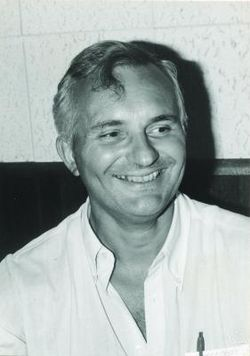
\includegraphics[width=\linewidth]{figures/lions.jpg}
    \captionof*{figure}{\tiny J.L. Lions}
  \end{minipage}}%
  \hfill
  \begin{minipage}[b]{0.46\textwidth}
    \includegraphics[width=\linewidth]{figures/stampacchia.jpg}
    \captionof*{figure}{\tiny G. Stampacchia}
  \end{minipage}
\end{figure}\vspace{-6ex}
\begin{figure}
	\centering
	\begin{tikzpicture}
		\node at (-4.2,1.2) {\scriptsize 
	    	$u$};
		\node at (-3.35,0) {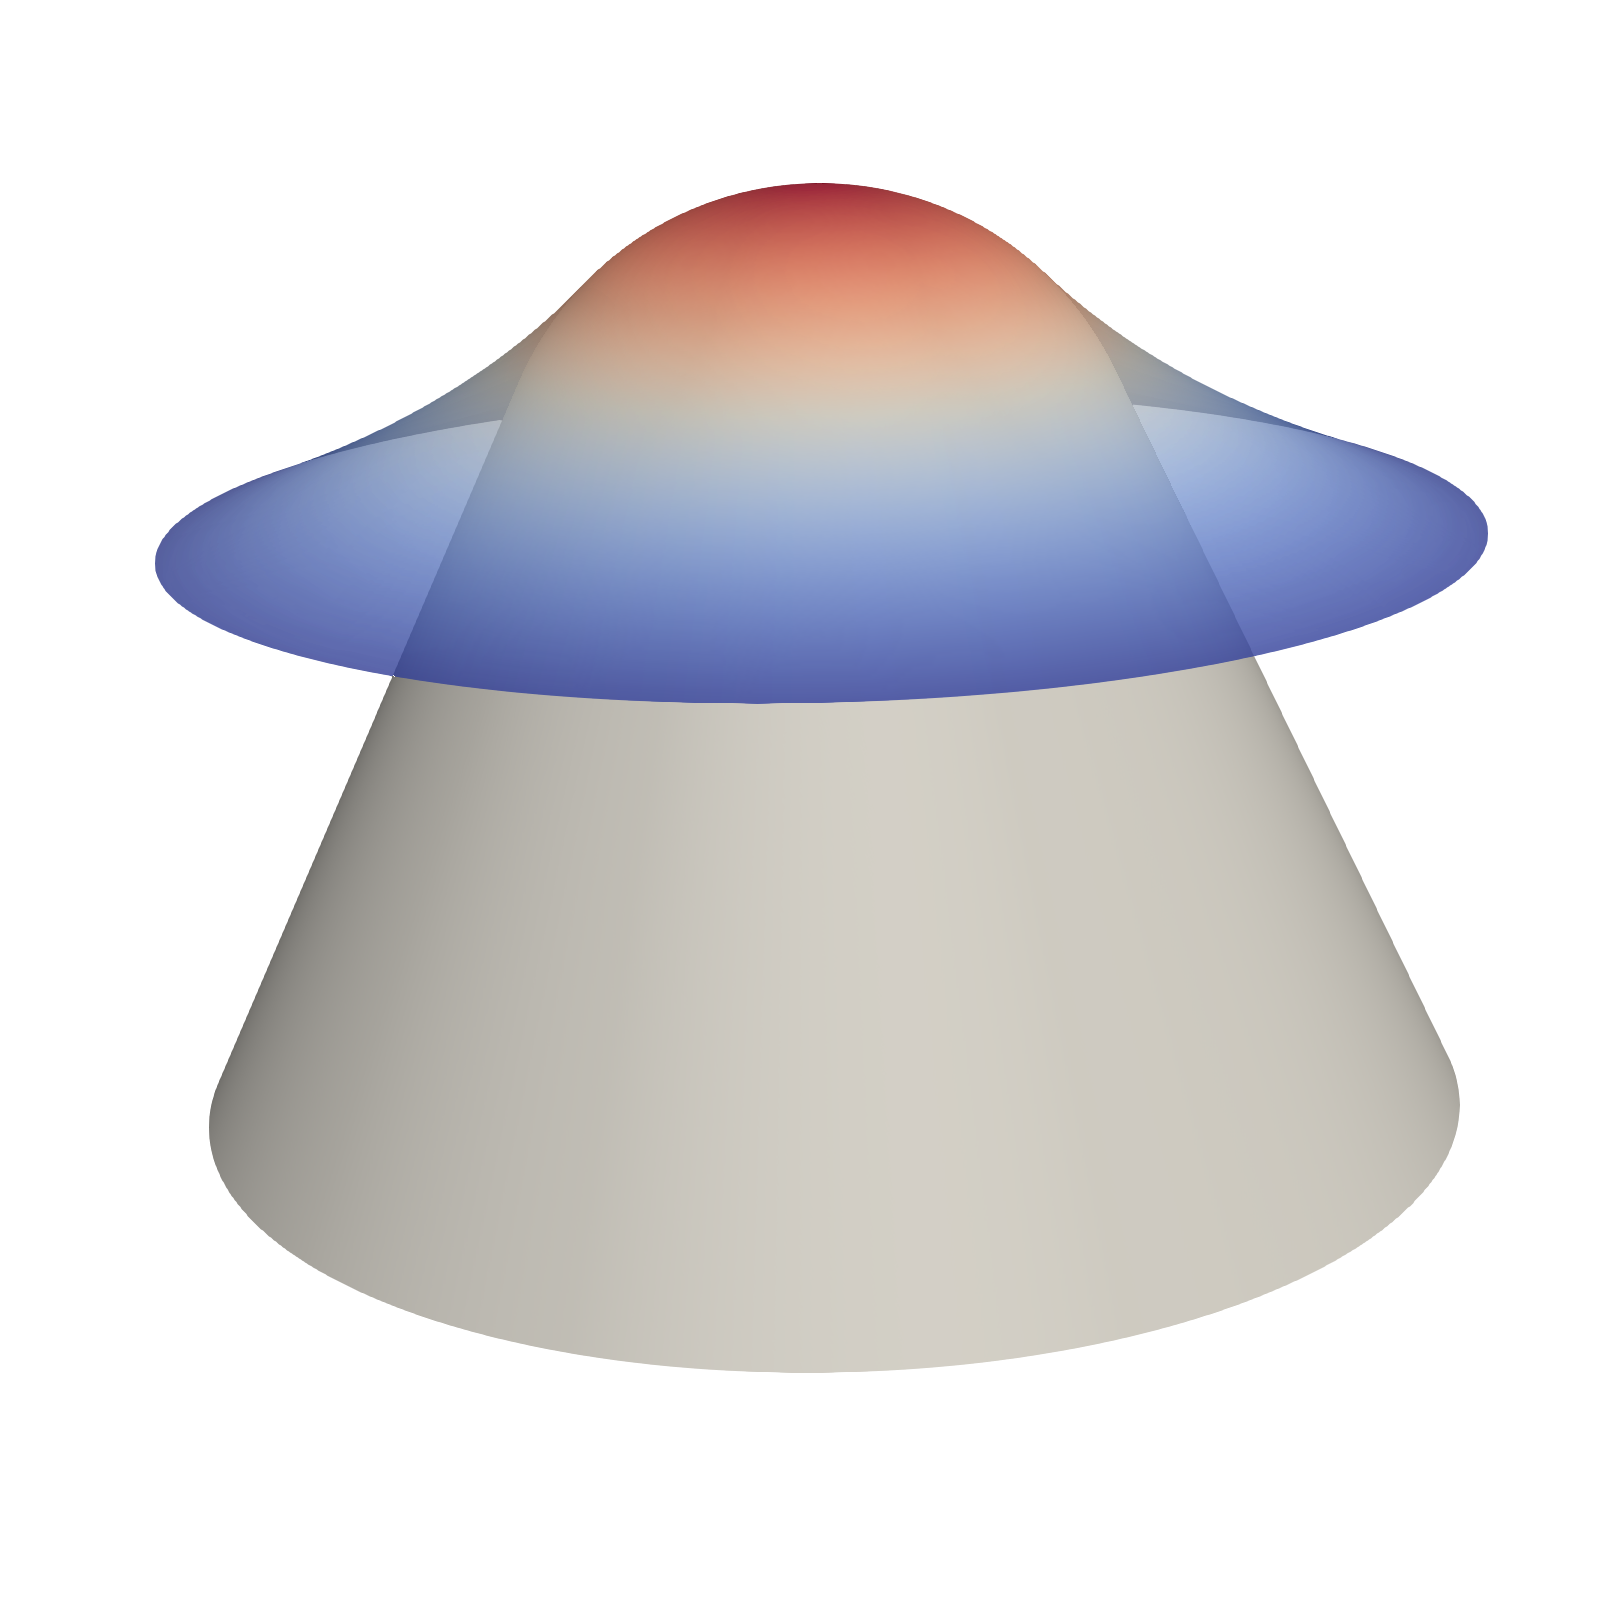
\includegraphics[height=1.25in]{figures/obstacle_new.png}};
		\node at (-2.2,-1.35) {\scriptsize 
	    	$\varphi$};
    \end{tikzpicture}

\end{figure}
\end{minipage}
\end{frame}

\begin{frame}\frametitle{The Lions-Stampacchia Theorem}
\begin{minipage}{0.6\linewidth}
\begin{beamercolorbox}[rounded=true, shadow=true, wd=\textwidth]{block body}
Comments:

\begin{itemize}
\item \visible<1->{For \textbf{symmetric $a$}, use the direct method.}
\item \visible<2->{For \textbf{nonsymmetric $a$}: The proof embeds the nonsymmetric problem in a parametric fixed point iteration of the type $u = S_{\rho}(v)$ with parameter $\rho > 0$.}
\item \visible<3->{The evaluation of $S_{\rho}(v)$ involves the solution of a related symmetric problem, which has a unique solution.}
\item \visible<4->{After deriving several key estimates, it becomes clear what $\rho$ needs to be to ensure $S_{\rho}(v)$ is a contraction.}
\end{itemize}

 \end{beamercolorbox}
\end{minipage}\hspace{4ex}
\begin{minipage}{0.3\linewidth}
 \centering
 \begin{figure}
  \centering\vspace{1ex}
  \visible<1->{\begin{minipage}[b]{0.45\textwidth}
    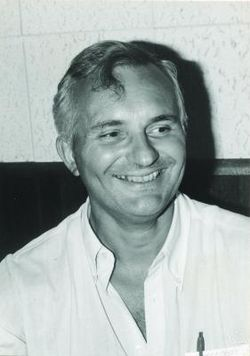
\includegraphics[width=\linewidth]{figures/lions.jpg}
    \captionof*{figure}{\tiny J.L. Lions}
  \end{minipage}}%
  \hfill
  \begin{minipage}[b]{0.46\textwidth}
    \includegraphics[width=\linewidth]{figures/stampacchia.jpg}
    \captionof*{figure}{\tiny G. Stampacchia}
  \end{minipage}
\end{figure}\vspace{-6ex}
\begin{figure}
	\centering
	\begin{tikzpicture}
		\node at (-4.2,1.2) {\scriptsize 
	    	$u$};
		\node at (-3.35,0) {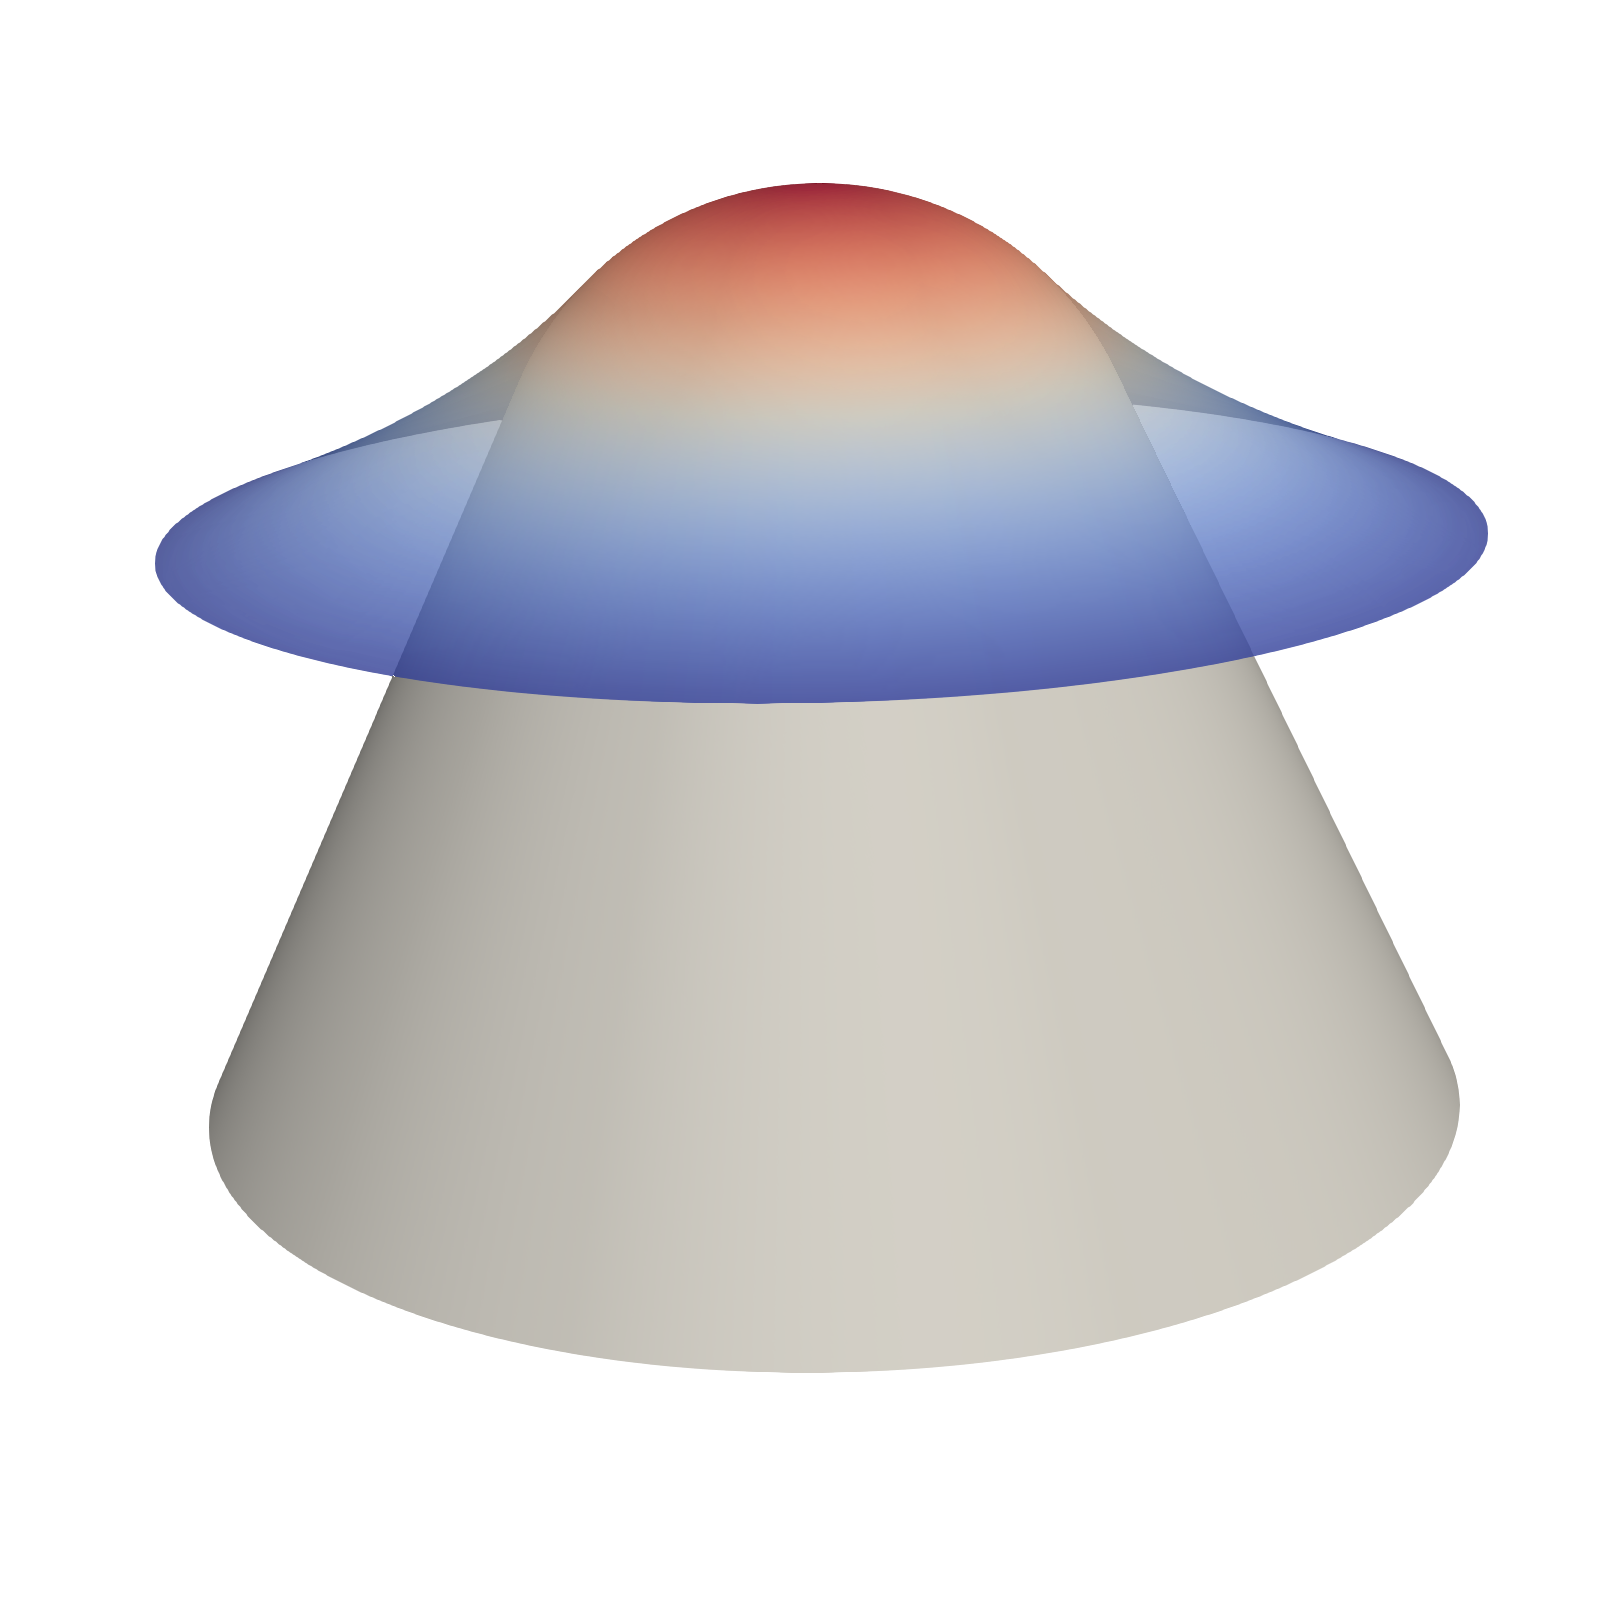
\includegraphics[height=1.25in]{figures/obstacle_new.png}};
		\node at (-2.2,-1.35) {\scriptsize 
	    	$\varphi$};
    \end{tikzpicture}

\end{figure}
\end{minipage}
\end{frame}

\section{Lagrange Multipliers}\label{sec:complementarity}
\begin{frame}\frametitle{Lagrange Multipliers}
\begin{beamercolorbox}[rounded=true, shadow=true, wd=\textwidth]{block title}\centering
 \visible<1->{What distinguishes these problems from ordinary PDEs?}
 \end{beamercolorbox}
 
  \visible<2->{
 \begin{beamercolorbox}[rounded=true, shadow=true, wd=\textwidth]{block body}
Consider again the VI for the Obstacle Problem: Find $u \in K$ such that
 \[
 (\nabla u, \nabla [v-u])_{L^2} \ge  (f,v-u)_{L^2} \quad \forall v \in K.
 \]
 
 \visible<3->{
Note that $a(u,v) :=  (\nabla u, \nabla v)_{L^2}$ is a symmetric bounded continuous bilinear form.\medskip

}\visible<4->{
Riesz Representation Theorem: There exists (symmetric) bounded linear operator $A : V \to V^*$:
 \[
 a(u,v) = \langle Au,v\rangle\quad \forall u,v \in V.
 \]
 We then view the VI more abstractly: Find $u \in K$ such that
 \[
 \langle Au - f, v - u \rangle_{V^*,V} \ge 0 \quad \forall v \in K
 \]\vspace{-3ex}
 }
 \end{beamercolorbox}}
\end{frame}

\begin{frame}\frametitle{Lagrange Multipliers} 
  \visible<1->{
 \begin{beamercolorbox}[rounded=true, shadow=true, wd=\textwidth]{block body}
Introduce a \alert{slack variable} $\lambda := Au - f$ and consider the problem: Find $(u,\lambda) \in K \times V^*$:
\[\aligned
Au - \lambda &= f \quad\text{ in } V^*\\
\langle \lambda,v-u \rangle_{V^*,V} &\ge 0 \quad \forall v \in K.
\endaligned
\]
 \visible<2->{
What more can we say about $\lambda$?\medskip

}\visible<3->{
\begin{enumerate}
\item \visible<3->{$u \in K$ and $w \in H^1_0(\Omega)$ with $w \ge 0$ $\Rightarrow$ $u + w \ge \varphi$ and $(u + w)|_{\Gamma} = g$.}
\item \visible<4->{Setting $v = u + w$ implies $\langle \lambda, w \rangle \ge 0$ for all $w \in H^1_0(\Omega)$ : $w \ge 0$. \alert{``$\lambda \ge 0$''}.}
\item \visible<5->{The Riesz-Schwarz theorem states $\lambda$ is in fact a nonnegative Radon measure on $\Omega$.}
\item \visible<6->{Kinderlehrer-Stampacchia Thm. 6.9: 
$
\mathrm{supp} \lambda \subset \mathcal{A} := \left\{x \in \Omega : u(x) = \varphi(x)\right\}.
$\\
Proof uses smooth bump functions at points in $\mathcal{A}$ to get clever test functions.
}
\end{enumerate}
 }
 \end{beamercolorbox}}
\end{frame}

\begin{frame}\frametitle{Lagrange Multipliers}
\begin{beamercolorbox}[rounded=true, shadow=true, wd=\textwidth]{block title}\centering
 \visible<1->{What does this have to do with what I learned in nonlinear optimization class!?}
 \end{beamercolorbox}

\begin{beamercolorbox}[rounded=true, shadow=true, wd=\textwidth]{block body}
 \visible<2->{If everything were in $\mathbb R^n$, we would have 
 \begin{enumerate}
 \item \visible<3->{$u_i \ge \varphi_i$ for a $i = 1,\dots,n$.}
 \item \visible<4->{For each $i = 1,\dots, n$, there would exist a \alert{Lagrange multiplier} $\lambda_i \ge 0$.}
 \item \visible<5->{For each $i = 1,\dots, n$, we would have a \alert{complementarity condition}:
$
 \lambda_i (u_i - \varphi_i) = 0.
$}
 \item \visible<6->{1. and 2. correspond to $u \in K$ and $\lambda \ge 0$ in the sense of $V^*$.}
 \item \visible<7->{The support condition means: Letting $\mathcal{I} := \left\{x \in \Omega : u(x) > \varphi(x)\right\}$ (\alert{inactive set})
 \[
 \int_{\mathcal{I}} \dd \lambda =  \lambda(\mathcal{I}) = \lambda(\left\{x \in \Omega : u(x) > \varphi(x)\right\}) = 0, 
 \]}\visible<8->{which is exactly what we get from the complementarity condition for $i$: $u_i > \varphi_i$.}
 \end{enumerate}}
 \end{beamercolorbox}
\end{frame}

\begin{frame}\frametitle{Lagrange Multipliers: Final Words}
\begin{beamercolorbox}[rounded=true, shadow=true, wd=\textwidth]{block body}
 \visible<1->{If $u \in H^2(\Omega)$, then $Au - f \in L^2(\Omega)$ so $\lambda$ will have a \alert{pointwise} description:
 \[
 \lambda = \max\{0, \lambda - c (u - \varphi) \} \quad \text{ for any constant } c > 0
 \]}\vspace{-3ex}
 
 \visible<2->{In this setting, the set of $x \in \Omega$ where $\lambda = 0$ and $u = \varphi$ holds is called the \alert{biactive set}.\medskip
 
 }\visible<3->{A \alert{non-negligible biactive set} typically leads to worst-case convergence rates.\medskip
 
 
 } \visible<4->{In $H^1(\Omega)$, we \alert{cannot ignore $(n-1)$-dimensional subsets} of $\Omega$ on which $u(x) = \varphi(x)$.}
 \end{beamercolorbox}
 
 \visible<5->{
 \begin{beamercolorbox}[rounded=true, shadow=true, wd=\textwidth]{block title}
 For the general setting $\{\min J(u) \text{ over } V : G(u) \in C\}$ we get optimality conditions like
 \[
 0 = dJ(u) +  d\langle \lambda, G(\cdot) \rangle(u)
 \]
 with $\lambda \in N_{C}(G(u)):= \left\{\mu : \langle \mu, y - G(u) \rangle \le 0 \quad \forall y \in C\right\}$.
  \end{beamercolorbox}
  }
\end{frame}

\section{Solving Variational Inequalities}\label{sec:algorithms}
%\begin{frame}{Algorithms}
%    \begin{enumerate}
%        \item Penalty
%        \item Barrier
%        \item Augmented Lagrangian
%    \end{enumerate}
%\end{frame}

\begin{frame}\frametitle{Towards Solution Algorithms}
\begin{beamercolorbox}[rounded=true, shadow=true, wd=\textwidth]{block body}\centering
 \visible<1->{How does one actually \alert{solve} a variational inequality?}
 \end{beamercolorbox}\hfill
 \visible<2->{
% \begin{minipage}{0.6\textwidth}
 \begin{beamercolorbox}[rounded=true, shadow=true, wd=\textwidth]{block body}\centering
 First Idea: Use a Ritz-Galerkin approach by replacing $V$ by $V_{h}$. Then use a black box optimization solver, e.g., active set method. 
 \end{beamercolorbox}}
 \hfill
  \visible<3->{
% \begin{minipage}{0.6\textwidth}
 \begin{beamercolorbox}[rounded=true, shadow=true, wd=\textwidth]{block title}\centering
What might be the issues with such an approach?
 \end{beamercolorbox}}
% \end{minipage}}%\quad\quad
% %
% \begin{minipage}{0.33\textwidth}\vspace{3ex}
%% \begin{beamercolorbox}[rounded=true, shadow=true, wd=\textwidth]{block body}
% \centering\visible<3->{
% \resizebox{\textwidth}{\textwidth}{%
%\begin{tikzpicture}
%\begin{axis}[
%%    width=\linewidth,
%%    height=4cm,
%    scale only axis,
%    axis lines=middle,
%    xlabel={$x$},
%    ylabel={$\phi_i(x)$},
%    xtick={0, 0.5, 1},
%    xticklabels={$x_0$, $x_1$, $x_2$},
%    ytick={-0.5, 0, 0.5, 1},
%    ymin=-0.6, ymax=1.2,
%    xmin=0, xmax=1,
%    legend style={font=\tiny, at={(1.0,-0.1)}, anchor=north east},
%    grid=major,
%    domain=0:1,
%    samples=200
%]
%
%\addplot[red, thick, dashed] {2*(x - 0.5)*(x - 1)};
%\addlegendentry{$\phi_0(x)$}
%
%\addplot[blue, thick] {-4*x*(x - 1)};
%\addlegendentry{$\phi_1(x)$}
%
%\addplot[green!60!black, thick, dashdotted] {2*x*(x - 0.5)};
%\addlegendentry{$\phi_2(x)$}
%
%\end{axis}
%\end{tikzpicture}
%}}
%% \end{beamercolorbox} 
% \end{minipage}
 
 \end{frame}
 
 \begin{frame}\frametitle{Potential Issues}
   \visible<1->{
 \begin{beamercolorbox}[rounded=true, shadow=true, wd=\textwidth]{block title}\centering
Black box optimization solvers typically use the Euclidean inner product for computing gradients. Why is that a problem?
 \end{beamercolorbox}}
 
 \visible<2->{
 \begin{beamercolorbox}[rounded=true, shadow=true, wd=\textwidth]{block body}
Consider 
$
J(u) := \frac{1}{2} \| \nabla u \|^2_{L^2(\Omega)} - (f,u)_{L^2(\Omega)}  \text{ with } u \in H^1_0(\Omega), f \in L^2(\Omega).
$
\visible<3->{The \alert{derivative} in $H^1_0(\Omega)$ in $u$ in direction $\delta \in H^1_0(\Omega)$ is:
\[
dJ(u)\delta = (\nabla u, \nabla \delta)_{L^2(\Omega)} - (f,\delta)_{L^2(\Omega)}.
\]
The derivative is a \alert{dual quantity}, i.e., an element of $H^{-1}(\Omega)$. }\visible<4->{But the Riesz Rep.\ Thm.\, says the \alert{gradient} $\nabla J(u)$ is the unique solution $y$ to
\[
(\nabla y, \nabla \varphi)_{L^2(\Omega)} = (\nabla u, \nabla \varphi)_{L^2(\Omega)} - (f,\varphi)_{L^2(\Omega)} \quad \forall \varphi \in H^1_0(\Omega).
\]}\visible<5->{
E.g. $f \equiv 0$ implies $\nabla J(u) = u$. In general, $\nabla J(u) = u - (-\Delta)^{-1} f.$}
 \end{beamercolorbox}}
 \end{frame}
 
  \begin{frame}\frametitle{Potential Issues}
    \visible<1->{
 \begin{beamercolorbox}[rounded=true, shadow=true, wd=\textwidth]{block body}
If we ``\alert{first discretize, then optimize}'', then we feed the solver a discretized objective
\[
J_h(\mathbf{u}) := \frac{1}{2} \mathbf{u}^T A_h \mathbf{u} - \mathbf{f}^T M_h \mathbf{u}\quad \text{ with }\quad \mathbf{u}, \mathbf{f} \in \mathbb R^n,
\]
with mesh parameter $h > 0$, whose gradient in $\mathbb R^n$ is given by
\[
\nabla^{\mathbb R^n} J_h(\mathbf{u}) := A_h \mathbf{u} - M_h \mathbf{f}.
\]
\visible<2->{Let $\mathbf{f} \equiv 0$. Now the gradient is $A_h \mathbf{u}$, where  \alert{the condition number of $A_h$ is $O(h^{-2})$!}\medskip 
}

\visible<3->{The gradient associated with the finite dimensional subspace $V_h$, however, should be
 \[
\nabla^{V_h} J_h(\mathbf{u}) := A^{-1}_h(A_h \mathbf{u} - M_h \mathbf{f}) = \mathbf{u} - A^{-1}_h M_h \mathbf{f},
\]
which fixes the conditioning. Most solvers do not do this automatically. 
}

 \end{beamercolorbox}}
 \end{frame}
 
\begin{frame}\frametitle{Potential Issues}

\begin{minipage}{0.55\linewidth}
 \begin{beamercolorbox}[rounded=true, shadow=true, wd=\textwidth]{block body}
 \visible<1->{Recall the 
 \textbf{mixed complementarity problem}:}\medskip
 
 \visible<1->{Find $(u,\lambda) \in H^1_0(\Omega) \times H^{-1}(\Omega)$ s.t.
\[
\underbrace{-\Delta u - \lambda = f,}_{\text{PDE}} \quad \underbrace{u \ge 0 \quad {\color{red}``\lambda \ge 0"} \quad \langle \lambda, u \rangle = 0}_{\text{Complementarity Condition}}.
\]}
 \end{beamercolorbox}
\end{minipage}\quad
\begin{minipage}{0.4\linewidth}
\centering\visible<1->{
	\begin{tikzpicture}
		\node at (-1.35,1.25) {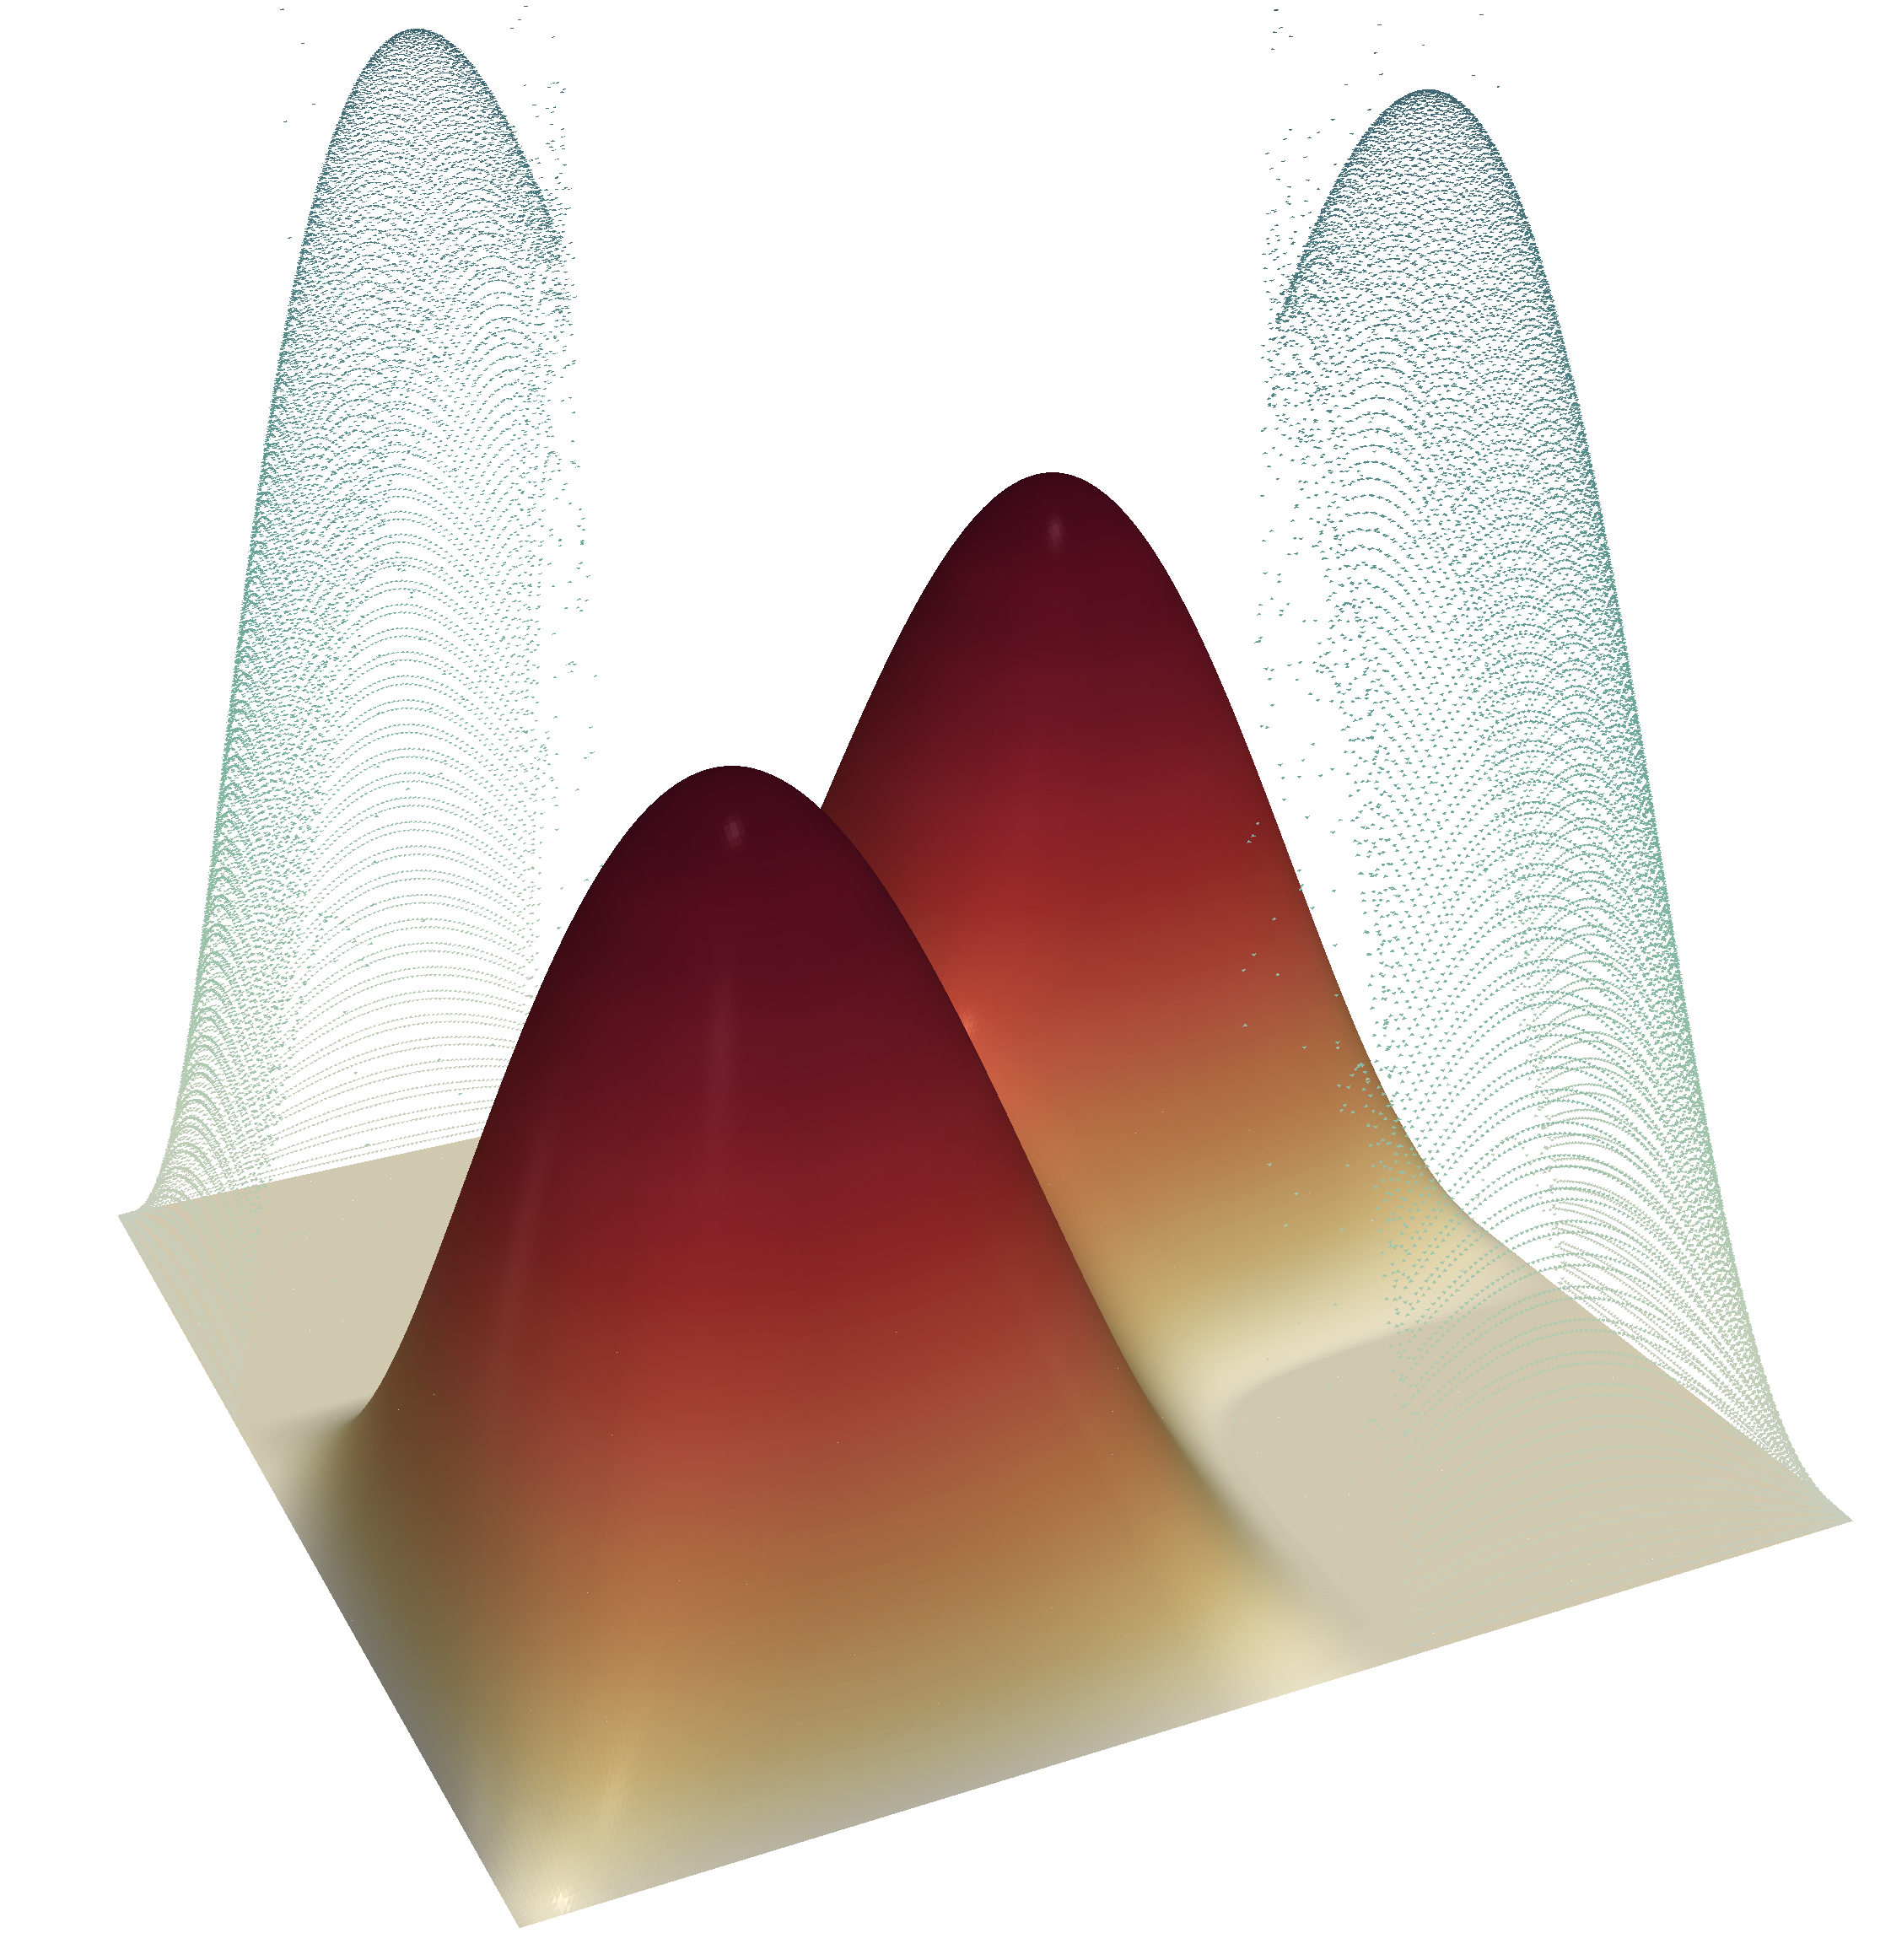
\includegraphics[clip=true, trim= 4cm 0 0 0, height=4cm]{figures/ObstacleExperiment2.png}};
		% \node at (-3.35,1) {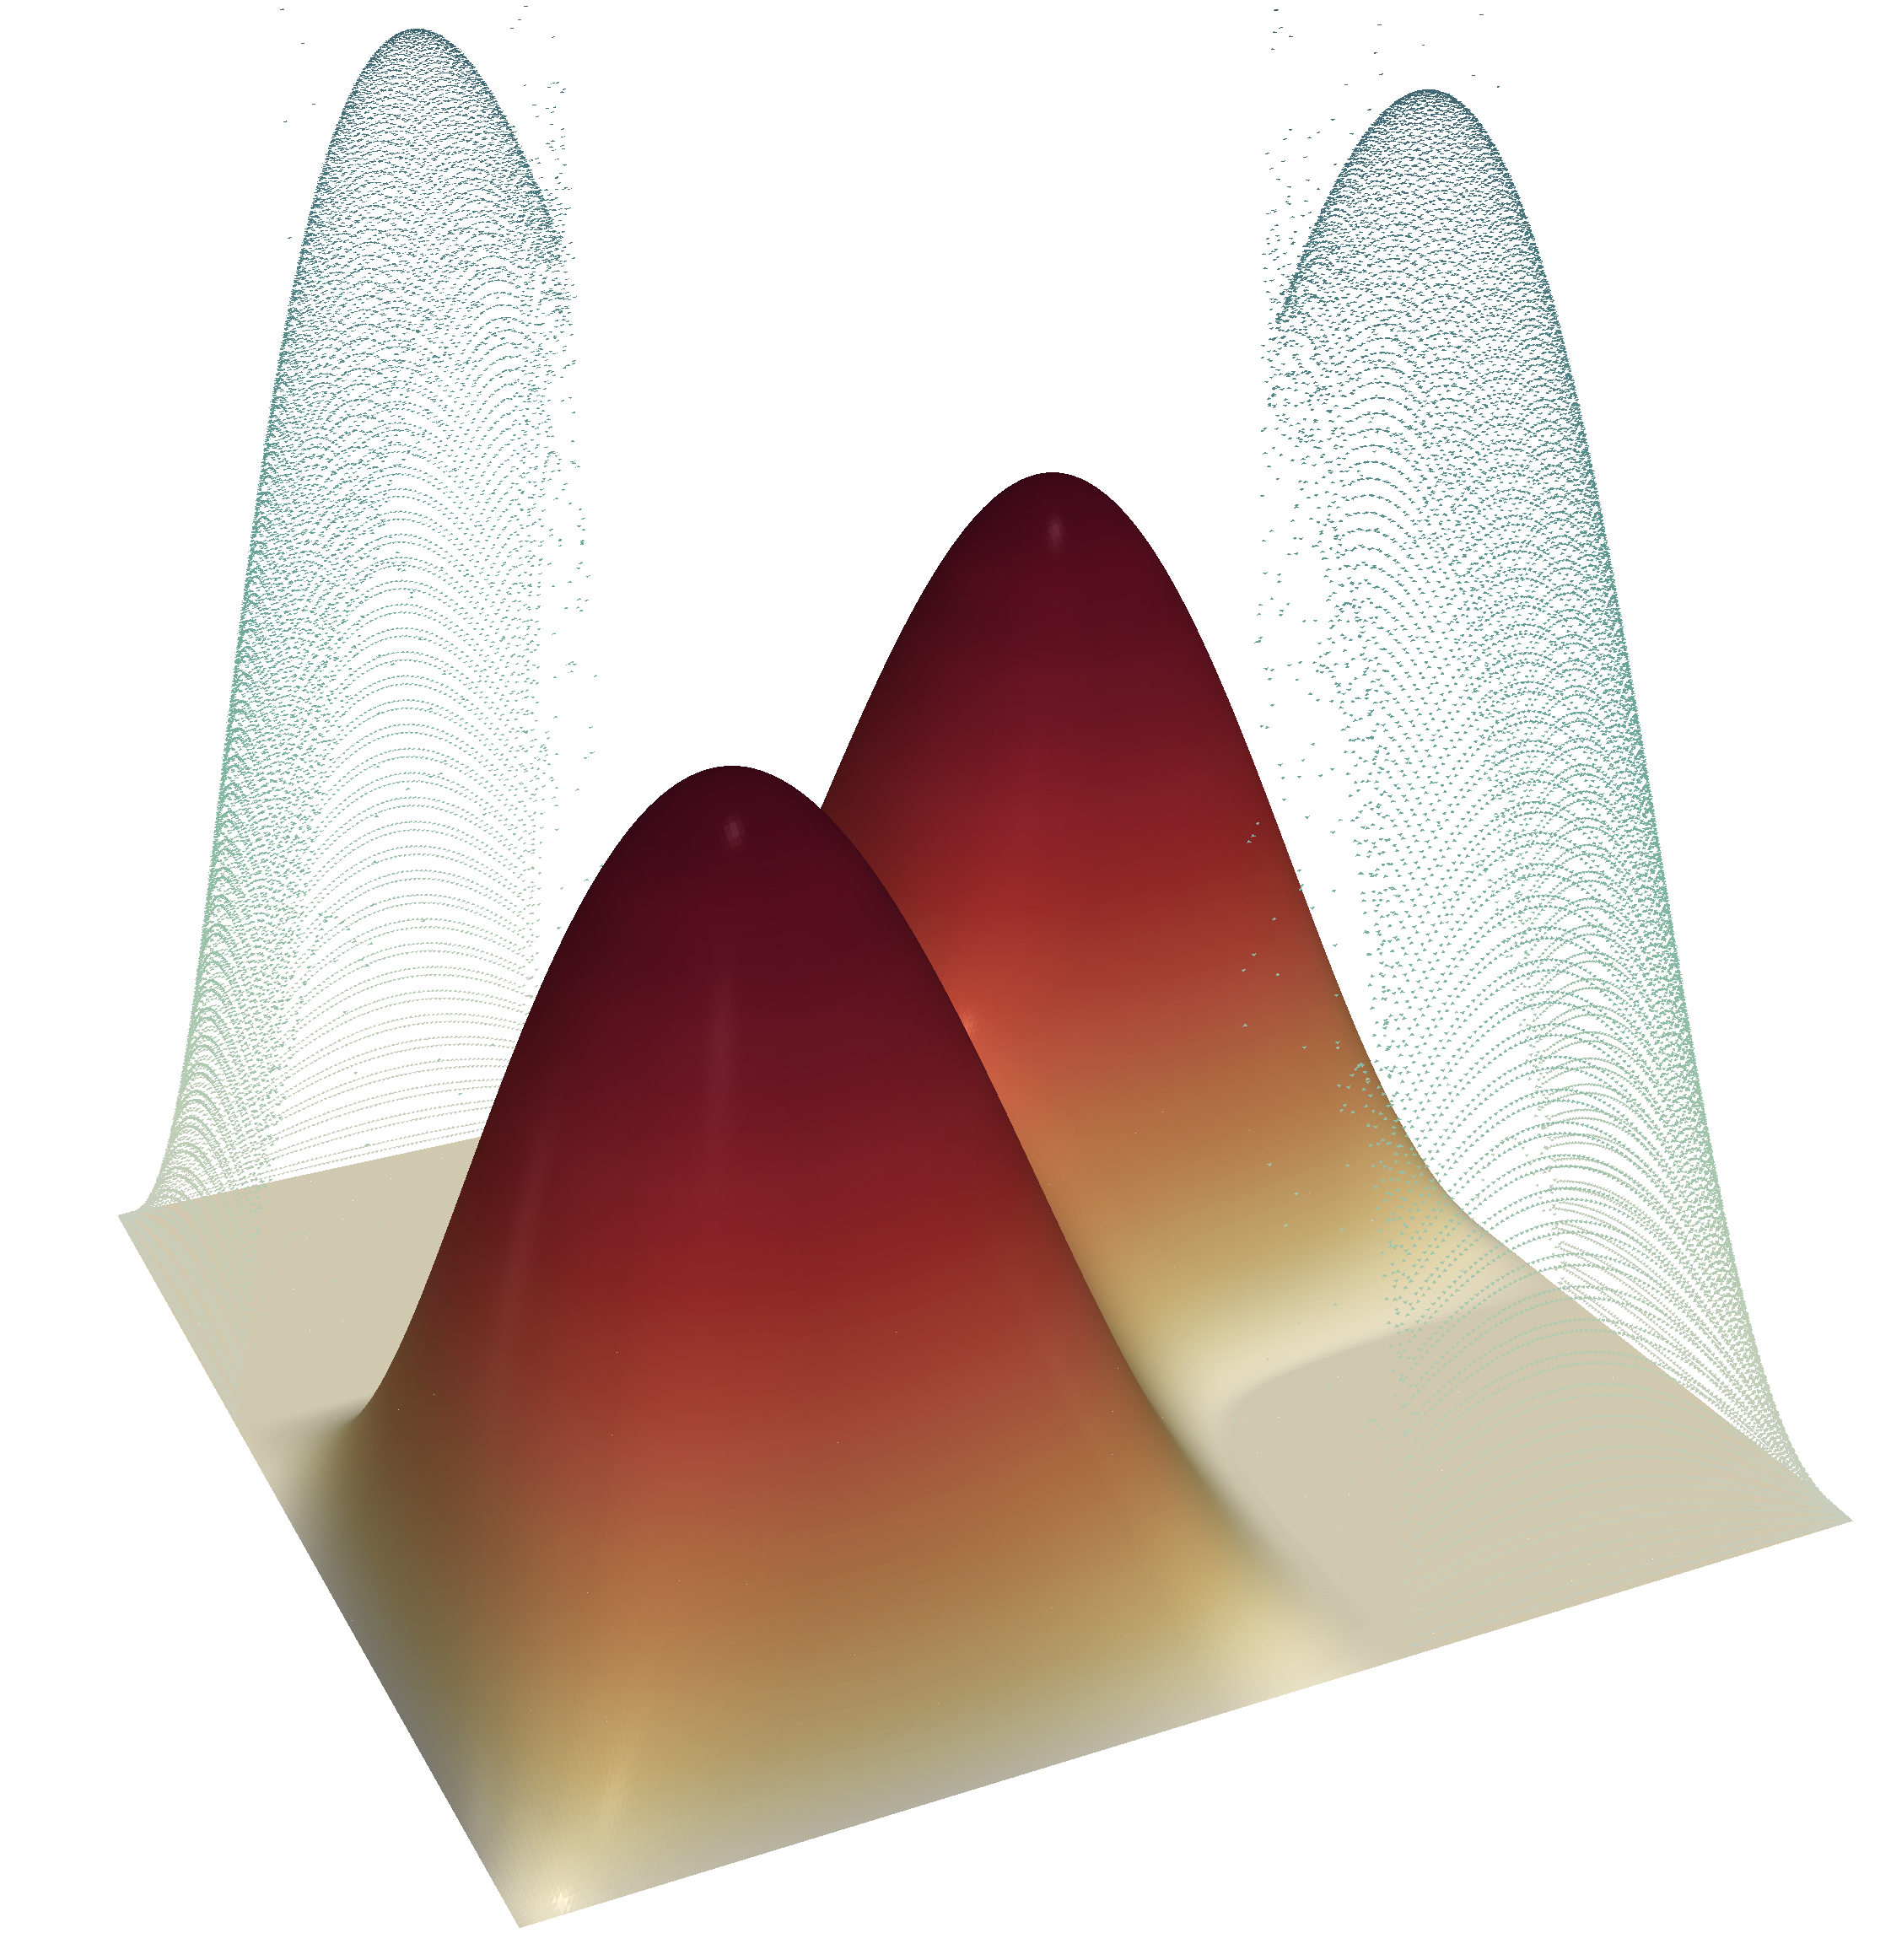
\includegraphics[clip=true, trim= 4cm 0 0 0, width=0.44\textwidth]{Figures/ObstacleExperiment2.png}};
%		\node at (3,0.4) {
%		   \includegraphics[clip=true, trim= 0 0 0.35cm 0, height=2.1in]{Figures/tikz/FEniCS_plots/example1/example1_ConvergenceRate.pdf}
%		};
	    % \node at (-4,2.8) {\includegraphics[height=2cm]{Figures/tikz/FEniCS_plots/example1/colorbar/colorbar1.pdf}};
	    \node at (-3.7,0.5) {\includegraphics[height=2cm]{figures/colorbar1.pdf}};
	    \node at (0.75,2.2) {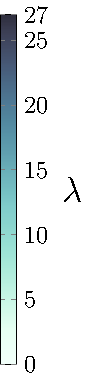
\includegraphics[height=2cm]{figures/colorbar2.pdf}};
    \end{tikzpicture}
}
\end{minipage}\medskip

\visible<2->{
%\begin{minipage}{0.48\linewidth}
\begin{beamercolorbox}[rounded=true, shadow=true, wd=\textwidth]{block body}
The \alert{low regularity of the Lagrange multiplier} will result in a numerical method that requires more iterations to reach the same stopping tolerance on increasingly finer meshes. This is known as \alert{mesh dependence}.
%$\lambda$ has low regularity. 
% 
%This results in \textit{mesh dependence}
%%\footnote{\tiny The number of iterations needed to reach the same stopping tolerance increases with mesh refinements.} 
% for methods tacitly requiring $\lambda \in L^2(\Omega)$.
\end{beamercolorbox}
%\end{minipage}
}
%\visible<5->{
%\begin{minipage}{0.48\linewidth}
% \begin{beamercolorbox}[rounded=true, shadow=true, wd=\textwidth]{block title}
%$\text{Leb}(\left\{x \in \Omega : u(x) = 0,\; \lambda(x) = 0 \right\}) > 0$ causes numerical instabilities.
%
%\centering
%``Loss of strict complementarity''
%\end{beamercolorbox}
%\end{minipage}
%}


\end{frame}
 
 \begin{frame}\frametitle{Potential Issues}
   \begin{beamercolorbox}[rounded=true, shadow=true, wd=\textwidth]{block title}\centering
  Can we faithfully discretize the inequality constraints?
   \end{beamercolorbox}
 \visible<2->{
 \begin{minipage}{0.6\textwidth}
 \begin{beamercolorbox}[rounded=true, shadow=true, wd=\textwidth]{block body}
\visible<2->{
Brezis \& Stampacchia (1968): The regularity theory for the obstacle problem is very similar to Poisson.\medskip 

$u \in H^2(\Omega)$ can be expected if $\Gamma$, $f$, and $\varphi$ are sufficiently regular.
}
\end{beamercolorbox}
\visible<3->{   
\begin{beamercolorbox}[rounded=true, shadow=true, wd=\textwidth]{block body}  
\visible<3->{This opens the door for higher order bases, $hp$-refinement, etc. \alert{However,...}
}

\visible<4->{ \medskip
If the basis elements are not non-negative, then the discrete solution $u_{h}$ will not be globally feasible!
 }
 \end{beamercolorbox}}
 \end{minipage}}\quad\quad
 %
 \begin{minipage}{0.3\textwidth}\vspace{3ex}
% \begin{beamercolorbox}[rounded=true, shadow=true, wd=\textwidth]{block body}
 \centering\visible<3->{
 \resizebox{\textwidth}{\textwidth}{%
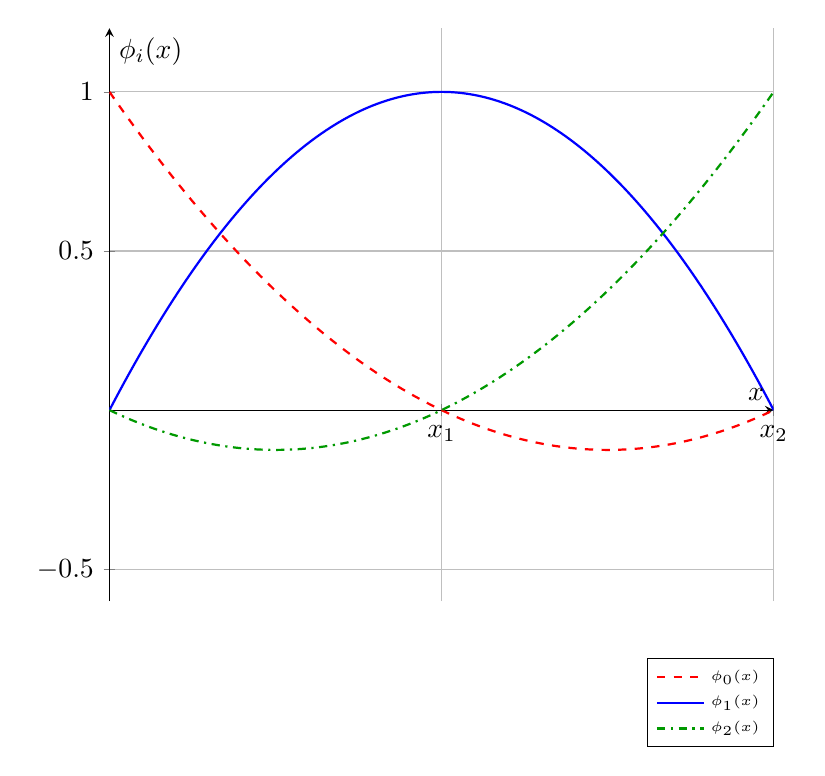
\begin{tikzpicture}
\begin{axis}[
%    width=\linewidth,
%    height=4cm,
    scale only axis,
    axis lines=middle,
    xlabel={$x$},
    ylabel={$\phi_i(x)$},
    xtick={0, 0.5, 1},
    xticklabels={$x_0$, $x_1$, $x_2$},
    ytick={-0.5, 0, 0.5, 1},
    ymin=-0.6, ymax=1.2,
    xmin=0, xmax=1,
    legend style={font=\tiny, at={(1.0,-0.1)}, anchor=north east},
    grid=major,
    domain=0:1,
    samples=200
]

\addplot[red, thick, dashed] {2*(x - 0.5)*(x - 1)};
\addlegendentry{$\phi_0(x)$}

\addplot[blue, thick] {-4*x*(x - 1)};
\addlegendentry{$\phi_1(x)$}

\addplot[green!60!black, thick, dashdotted] {2*x*(x - 0.5)};
\addlegendentry{$\phi_2(x)$}

\end{axis}
\end{tikzpicture}
}}
% \end{beamercolorbox} 
 \end{minipage}
 \visible<5->{
  \begin{beamercolorbox}[rounded=true, shadow=true, wd=\textwidth]{block title}\centering
Non-negativity is not enough: There are linear combinations of Bernstein polynomials that are globally nonnegative but which have some negative coefficients!
   \end{beamercolorbox}
 }
\end{frame}


 \begin{frame}\frametitle{Summary}
      \begin{beamercolorbox}[rounded=true, shadow=true, wd=\textwidth]{block body}
An \alert{\bf{ideal solver}} is...\medskip

%\begin{enumerate}
%\item 
...designed in accordance with the infinite-dimensional nature of the problem.\medskip

%\item 
...provably (or observably) mesh independent for standard stopping criteria.\medskip

%\item 
...able to provide a globally constraint-preserving representation of $u$ (or $G(u)$ in general).
%\end{enumerate}
 \end{beamercolorbox}
 \hfill
\visible<2->{
 \begin{beamercolorbox}[rounded=true, shadow=true, wd=\textwidth]{block body}
From a \alert{\bf{practical standpoint}}, an \alert{\bf{ideal solver}} should be...\medskip 
%\begin{enumerate}
%\item 

...fast to converge.\medskip

%\item 
...have a low computational cost per iteration.\medskip

%\item 
...easy to implement
%\end{enumerate}
   \end{beamercolorbox}}
 \end{frame}

\begin{frame}\frametitle{Summary}
\begin{beamercolorbox}[rounded=true, shadow=true, wd=\textwidth]{block body}
\begin{enumerate}
\item Starting with a classical problem from the theory of linear elliptic partial differential equations, we introduced the Direct Method of the Calculus of Variations.
\item By restricting the solution space to pointwise inequality constraints, we motivated the necessity of the study of variational inequalities, which enjoy a wide array of interesting applications.
\item We introduced the Obstacle Problem for the first time in order to understand how to derive variational inequalities and prove existence and uniqueness of solutions.
\item Lagrange Multipliers were introduced to highlight the differences  to the theory of PDEs and linearly constrained variational problems. The low regularity of the Lagrange multiplier was discussed.
\item The issues of poor scaling, mesh independence, and a lack of global bound preservation of naive solution algorithms is discussed.
\end{enumerate}
\end{beamercolorbox}
\end{frame}

% \begin{frame}{Frame Title}
    
% \end{frame}
% \begin{frame}{Frame Title}
    
% \end{frame}
% \begin{frame}{Frame Title}
    
% \end{frame}
% \section{}
% \begin{frame}{Frame Title}
    
% \end{frame}
% \begin{frame}{Frame Title}
    
% \end{frame}
% \begin{frame}{Frame Title}
    
% \end{frame}
% \begin{frame}{Frame Title}
    
% \end{frame}
% \begin{frame}{Frame Title}
    
% \end{frame}
% \section{}
% \begin{frame}{Frame Title}
    
% \end{frame}
% \begin{frame}{Frame Title}
    
% \end{frame}
% \begin{frame}{Frame Title}
    
% \end{frame}
% \begin{frame}{Frame Title}
    
% \end{frame}

\end{document}